\documentclass[10pt]{article}
\usepackage[utf8]{inputenc}
\usepackage[T1]{fontenc}
\usepackage{hyperref}
\hypersetup{colorlinks=true, linkcolor=blue, filecolor=magenta, urlcolor=cyan,}
\urlstyle{same}
\usepackage{amsmath}
\usepackage{amsfonts}
\usepackage{amssymb}
\usepackage[version=4]{mhchem}
\usepackage{stmaryrd}
\usepackage{bbold}
\usepackage{graphicx}
\usepackage[export]{adjustbox}
\graphicspath{ {./images/} }

\title{THE FOUR-EQUATION NEW KEYNESIAN MODEL }

\author{Eric Sims, Jing Cynthia Wu, and Ji Zhang*}
\date{}


%New command to display footnote whose markers will always be hidden
\let\svthefootnote\thefootnote
\newcommand\blfootnotetext[1]{%
  \let\thefootnote\relax\footnote{#1}%
  \addtocounter{footnote}{-1}%
  \let\thefootnote\svthefootnote%
}

%Overriding the \footnotetext command to hide the marker if its value is `0`
\let\svfootnotetext\footnotetext
\renewcommand\footnotetext[2][?]{%
  \if\relax#1\relax%
    \ifnum\value{footnote}=0\blfootnotetext{#2}\else\svfootnotetext{#2}\fi%
  \else%
    \if?#1\ifnum\value{footnote}=0\blfootnotetext{#2}\else\svfootnotetext{#2}\fi%
    \else\svfootnotetext[#1]{#2}\fi%
  \fi
}

\begin{document}
\maketitle


\begin{abstract}
This paper develops a New Keynesian model featuring financial intermediation, short- and long-term bonds, credit shocks, and scope for unconventional monetary policy. The log-linearized model reduces to four equations: Phillips and IS curves, as well as policy rules for the shortterm interest rate and the central bank's long-bond portfolio (QE). Credit shocks and QE appear in both the IS and Phillips curves. In equilibrium, optimal monetary policy entails adjusting the short-term interest rate to offset natural rate shocks but using QE to offset credit market disruptions. Use of QE significantly mitigates the costs of a binding zero lower bound.
\end{abstract}

\section*{I. Introduction}
THE textbook three-equation New Keynesian (NK) model (see, e.g., Woodford, 2003, or Galí, 2008) has enormous influence in both policy circles and among academic researchers due to its elegance and tractability. The model boils down to a forward-looking IS equation characterizing aggregate demand, a Phillips curve describing aggregate supply, and a rule for the central bank's principal policy tool, the short-term interest rate. The model has yielded several important insights, including the potential desirability of inflation targeting, the gains from policy commitment over discretion, and the importance of having the policy rate track the "natural" or "neutral" rate of interest.

In spite of its myriad uses, the textbook model has proven inadequate for examining a range of issues that have come to the fore in policy circles over the past decade. As it abstracts from the financial sector, the model is unable to address the consequences of financial market disruption of the sort that rocked the global economy from 2007 to 2009. It is also incapable of directly speaking to the potential benefits and costs of quantitative easing (QE) types of policies. QE policies were among the first and most prominent of several unconventional interventions deployed to fight the global financial crisis once policy rates were lowered to 0 . There is now a nascent literature incorporating QE into medium-scale dynamic stochastic general equilibrium (DSGE) models (Gertler \& Karadi, 2011, 2013; Carlstrom, Fuerst, \& Paustian, 2017; or Sims \& Wu, 2021). While this work has proven useful and generated several important insights, these quantitative frameworks lack the simplicity and transparency of the textbook three-equation model.

\footnotetext{Received for publication June 15, 2020. Revision accepted for publication June 3, 2021. Editor: Olivier Coibion.\\
*Sims and Wu: Notre Dame and NBER; Zhang: Tsinghua PBCSF.\\
We are grateful to Todd Clark, Oli Coibion, Drew Creal, Argia Sbordone, Peter Van Tassel, two anonymous referees, as well as seminar participants at the Federal Reserve Banks of Boston, Cleveland, New York, and San Francisco; University of California, Davis; Texas A\&M University; Purdue University; and the Toulouse School of Economics for helpful comments. This material is based on work supported by the National Science Foundation under grant SES-1949107.\\
A supplemental appendix is available online at \href{https://doi.org/10.1162/}{https://doi.org/10.1162/} rest\_a\_01071.
}Our paper bridges the gap between the complicated quantitative DSGE models that have been developed to study QE with the elegance and tractability of the textbook threeequation model. Our model incorporates financial intermediaries, short- and long-term bonds, credit market shocks, and scope for central bank bond holdings to be economically relevant. The linearized version of our model reduces to four, rather than three, key equations. The IS and Phillips curves are similar to the three-equation benchmark. The innovation is that credit shocks and central bank long bond holdings appear additively in both the IS and Phillips curves. This differs from many ad hoc treatments of financial disturbances, which often simply include residuals in the IS equation meant to proxy for credit spreads (Smets \& Wouters, 2007). The model is closed with a rule for the short-term policy rate (as in the benchmark three-equation model) and a rule for the central bank's long bond portfolio.

We study optimal monetary policy in the context of our four-equation model. Reflecting central banks' dual mandate, we focus on an objective function that minimizes a weighted sum of volatilities of inflation and the output gap. Because credit shocks appear in the Phillips curve, the so-called divine coincidence (Blanchard \& Galí, 2007) does not hold, and it is not possible to achieve the global minimum of the loss function with just one policy instrument.

When the central bank can actively manage both the shortterm interest rate and a bond portfolio, it can achieve complete stabilization of both inflation and the output gap. In equilibrium, optimal policy entails adjusting the short-term interest to track fluctuations in the natural rate of interest (as in the benchmark three-equation model), but adjusting the long bond portfolio to offset the effects of credit market disturbances. Our model therefore has an implication that differs from the conventional wisdom among policymakers that adjustment of short-term interest rates is sufficient to meet a dual mandate of price and output stability: in general, QE policies ought to be used all the time to counter credit market shocks, not only when policy rates are constrained by the zero lower bound (ZLB).

We also explore the implications of the ZLB for policy. When the policy rate is unavailable, optimal balance sheet policy is characterized by a "lean-against-the-wind" condition that nevertheless differs from the standard condition under discretion in the textbook three-equation model. A couple of interesting results emerge. First, credit market shocks need not have differential effects at the ZLB in comparison to normal times. Adjusting the long bond portfolio in exactly the same way as it would absent a ZLB constraint, the central bank is able to stabilize both inflation and the output gap in response to credit shocks at the ZLB. Second, QE policies can serve as an effective (albeit imperfect) substitute for conventional policy in response to natural rate shocks. Without QE\\
available, output and inflation react suboptimally to natural rate shocks when the short-term policy rate is constrained, the more so the longer the anticipated duration of the ZLB. A central bank can partially offset these nonoptimal responses by adjusting its long bond portfolio. We derive an analytical expression for the optimal equilibrium path for QE at the ZLB as a function of the relative welfare weight on the output gap in the loss function. Though it is not possible to completely stabilize both inflation and the gap, a central bank engaging in QE operations can significantly reduce the costs of the ZLB.

Our model has important implications for central banks facing a dual mandate to stabilize both inflation and real economic activity due to the failure of the divine coincidence. How much QE is desired at the ZLB depends critically on how much weight the central bank puts on inflation versus output fluctuations. The more weight the central bank puts on the output gap, the less QE is required in response to a shock to the neutral rate of interest. Prior to the Great Recession, active management of a long-bond portfolio was not a major feature of most central banks' toolkits, Japan being one notable exception.

With only one policy instrument available, a lean-against-the-wind condition for the policy rate holds; in fact, this condition is the same as in the textbook three-equation model. The direction for the optimal short rate response to a credit shock depends on whether the central bank cares more about inflation or output stabilization. For a positive credit shock, a central bank focusing solely on inflation would increase the short rate, whereas if the central bank only cares about the output gap, it would instead cut the short rate. Alternatively, if a central bank can use bond purchases all the time as a policy instrument, there need not be any conflict between the two aspects of the dual mandate.

Our analysis of optimal policy highlighted above studies how a central bank's two instruments (the policy rate and long bond portfolio) ought to optimally adjust in equilibrium to stabilize its two targets (inflation and the output gap). While instructive, targeting rules of this sort may not be easily implementable. We also therefore consider an extension with "simple and implementable" rules for both the policy rate and the bond portfolio (Schmitt-Grohe \& Uribe, 2007): both instruments follow Taylor-type rules that react to deviations in the two target variables (inflation and the output gap). When the long bond portfolio does not react to endogenous variables, the restrictions on parameter values of the rule for the policy rate necessary for equilibrium determinacy are identical to the standard three-equation model. When the long bond portfolio does react to endogenous variables, determinacy is more likely when it responds strongly to the output gap and not inflation. We then show that having the policy rate react strongly to inflation and the bond portfolio react strongly to the output gap mimics the optimal allocations while also delivering a determinant equilibrium. We further show that an implementable rule for the central bank's long bond portfo-\\
lio significantly ameliorates the adverse consequences of a binding ZLB on the policy rate.

Though irrelevant in a standard model (Wallace, 1981), there are several potential channels by which QE can transmit to the real economy that have been explored in the literature (see Bhattarai \& Neely, 2020, for a thorough survey). One is a signaling channel, wherein accumulating a large balance sheet in the present might commit a central bank to lower short-term policy rates in the future (Bauer \& Rudebusch, 2014, and Bhattarai, Eggertsson, \& Gafarov, 2019). Another is based on exogenous participation constraints that build on the preferred habitat theory of the term structure (Vayanos \& Vila, 2009; Hamilton \& Wu, 2012; Chen, Cúrdia, \& Ferrero, 2012). A third assumes leverage constraints on intermediaries (Gertler \& Karadi, 2011, 2013). The key friction in our model is a leverage constraint that allows for a long-short interest rate spread. Relative to more involved papers based on a leverage constraint, such as Sims and Wu (2021), our model makes a number of simplifying assumptions that allow us to reduce the model down to four equations. At the expense of some realism, these simplifying assumptions afford a great deal of tractability, which allows us to make clear statements about optimal policy. More expansive models with leverage constraints nevertheless generate similar quantitative predictions as our four-equation model.

Our paper relates to the literature on unconventional monetary policy in the New Keynesian model. Gertler and Karadi (2011, 2013), Carlstrom et al. (2017), Sims and Wu (2021, 2020b), and Mau (2019) all represent attempts to model largescale asset purchases in a quantitative DSGE framework. Distinct from this strand of the literature, one important contribution of our paper is to incorporate the financial frictions giving rise to effective QE policies in these papers into the tractable small-scale New Keynesian model of Clarida, Galí, and Gertler (1999) that is popular among academics and policymakers alike. The framework we present here can be used to address a number of important policy questions in a way similar to how the three-equation model is used. For example, Sims and Wu (2020a) use the four-equation model to relate the Fed's QE policies in the wake of the Great Recession to the Wu and Xia (2016) shadow rate series.

The remainder of the paper is organized as follows. Section II presents the model. Section III discusses optimal central bank policy. Section IV considers optimal implementable rules for both the policy rate and the central bank's long bond portfolio. Section V offers concluding thoughts.

\section*{II. Model}
This section presents our model. We first present the fourequation linearized model in section IIA. The full nonlinear model is derived from first principles in section IIB. Section IIC studies positive properties of a calibrated version of the model before turning to normative issues in section III. Details are available in online appendixes A to F.

\section*{A. The Four-Equation Model}
The principal equations of our linearized model are an IS curve,\\
\begin{align*}
x_{t}= & \mathbb{E}_{t} x_{t+1}-\frac{1-z}{\sigma}\left(r_{t}^{s}-\mathbb{E}_{t} \pi_{t+1}-r_{t}^{*}\right) \\
& -z\left[\bar{b}^{F I}\left(\mathbb{E}_{t} \theta_{t+1}-\theta_{t}\right)+\bar{b}^{c b}\left(\mathbb{E}_{t} q e_{t+1}-q e_{t}\right)\right], \tag{1}
\end{align*}\\
and a Phillips curve,

\begin{equation*}
\pi_{t}=\gamma \zeta x_{t}-\frac{z \gamma \sigma}{1-z}\left[\bar{b}^{F I} \theta_{t}+\bar{b}^{c b} q e_{t}\right]+\beta \mathbb{E}_{t} \pi_{t+1} \tag{2}
\end{equation*}

Lowercase variables with a $t$ subscript denote log deviations about the nonstochastic steady state. $\pi_{t}$ is inflation, and $x_{t}=y_{t}-y_{t}^{*}$ denotes the output gap, where $y_{t}^{*}$ is the equilibrium level of output consistent with price flexibility and no credit shocks. ${ }^{1}$ We refer to this level of output as potential output. Similarly, $r_{t}^{*}$ denotes the natural rate of interest, that is, the real interest rate consistent with output equaling potential. It follows an exogenous process. $\theta_{t}$ captures credit conditions in the financial market; positive values correspond to more favorable conditions. This variable is described further in section IIB. We take it to be exogenous and henceforth refer to it as a credit shock. $q e_{t}$ denotes the real market value of the central bank's long-term bond portfolio. $r_{t}^{s}$ is the shortterm nominal interest.

Letters without $t$ subscripts are parameters or steady-state values. $\sigma, \beta$, and $\gamma$ are standard parameters: $\sigma$ measures the inverse intertemporal elasticity of substitution, $\beta$ is a subjective discount factor, and $\gamma$ is the elasticity of inflation with respect to real marginal cost. ${ }^{2} \bar{b}^{F I}$ and $\bar{b}^{C B}$ are parameters measuring the steady-state long-term bond holdings of financial intermediaries and the central bank, respectively, relative to total outstanding long-term bonds. These coefficients sum to 1 : $\bar{b}^{F I}+\bar{b}^{C B}=1$.

As described in section IIB, there are two kinds of households in our model. We refer to these types of households as "parent" and "child," respectively. The parent is the standard household in a textbook New Keynesian model: it consumes, borrows, or saves via one-period bonds, supplies labor, and owns firms. The child does not supply labor and does not have an equity interest in production firms. It is less patient than the parent and finances its consumption by issuing long-term bonds. It pays the servicing cost of these long-term bonds with a transfer from the parent each period. The parameter

\footnotetext{${ }^{1}$ Traditionally in New Keynesian models, potential output is defined as the hypothetical level of output consistent with price flexibility and is denoted $y_{t}^{f}$. As described below, in our model, both price stickiness and financial frictions distort the competitive equilibrium. It is therefore natural to define potential output as a concept wherein both frictions are neutralized rather than just price rigidity. See further details in online appendix D.\\
${ }^{2}$ In particular, $\gamma=\frac{(1-\phi)(1-\phi \beta)}{\phi}$ is the standard expression in the threeequation model, where $\phi \in[0,1)$ measures the probability of nonprice adjustment.
}
$z \in[0,1)$ represents the share of children in the total population. $\zeta$ is the elasticity of real marginal cost with respect to the output gap; it is conceptually similar to the corresponding parameter in the standard three-equation model but augmented to account for two types of households. ${ }^{3}$ Our model collapses to the standard three-equation NK model when $z=0$. In this case, credit shocks and the central bank's long bond portfolio are irrelevant for the equilibrium dynamics of output and inflation.

Our four-equation New Keyneian model consists of equations (1) and (2), together with policy rules for the short-term interest rate $r_{t}^{s}$ and the central bank's long bond portfolio $q e_{t}$. Simple rule-based policies are specified in section IIC for positive analyses, whereas we discuss optimal policies in section III.

\section*{B. Derivation of the Four-Equation Model}
In this section, we present, from first principles, the economic environment giving rise to the linearized fourequation model laid out in section IIA. The economy is populated by the following agents: two types of households (parent and child), a representative financial intermediary, production firms, and a central bank. We discuss the problems of each below.

Note that we make several simplifying assumptions in this section in order to get the system to reduce to just four equations. This is intentional and for tractability. Nevertheless, the quantitative implications of our small-scale model are similar to more complicated models. For example, the dynamics of the child's consumption in our model are in line with the behavior of investment in Sims and Wu (2021). In online appendix F , we show some quantitative results when we relax a few of the assumptions that allow the system to reduce to four equations.

Parent. A representative parent receives utility from consumption, $C_{t}$ and disutility from labor, $L_{t}$. It discounts future utility flows by $\beta \in(0,1)$. Its lifetime utility is

\begin{equation*}
V_{t}=\max \mathbb{E}_{t} \sum_{j=0}^{\infty} \beta^{j}\left[\frac{C_{t+j}^{1-\sigma}-1}{1-\sigma}-\psi \frac{L_{t+j}^{1+\chi}}{1+\chi}\right] \tag{3}
\end{equation*}

$\sigma>0$ is the inverse elasticity of intertemporal substitution, $x \geq 0$ is the inverse Frisch elasticity, and $\psi>0$ is a scaling parameter.

The nominal price of consumption is $P_{t}$. The parent earns nominal income from labor, with a wage of $W_{t}$; receives dividends from ownership in firms and financial intermediaries, $D_{t}$ and $D_{t}^{F I}$, respectively; and receives a lump sum transfer from the fiscal authority, $T_{t}$. It can save via one-period

\footnotetext{${ }^{3}$ In our model, $\zeta=\frac{\chi(1-z)+\sigma}{1-z}$, where $\chi$ is the inverse Frisch labor supply elasticity for the parent. If $z=0, \zeta$ would be identical to the textbook threeequation model.
}
nominal bonds, $S_{t}$, that pay gross nominal interest rate $R_{t}^{s}$. In addition, it makes a transfer, $X_{t}^{b}$, to the child each period, as well as a transfer, $X_{t}^{F I}$, to financial intermediaries; though time varying, these are not choice variables. The parent's budget constraint is

\begin{align*}
& P_{t} C_{t}+S_{t} \leq W_{t} L_{t}+R_{t-1}^{s} S_{t-1}+P_{t} D_{t}+P_{t} D_{t}^{F I} \\
& +P_{t} T_{t}-P_{t} X_{t}^{b}-P_{t} X_{t}^{F I} \tag{4}
\end{align*}

The objective is to pick a sequence of consumption, labor, and one-period bonds to maximize equation (3) subject to the sequence of equation (4). The optimality conditions are standard:\\
\begin{align*}
\psi L_{t}^{\chi} & =C_{t}^{-\sigma} w_{t}  \tag{5}\\
\Lambda_{t-1, t} & =\beta\left(\frac{C_{t}}{C_{t-1}}\right)^{-\sigma},  \tag{6}\\
1 & =R_{t}^{s} \mathbb{E}_{t} \Lambda_{t, t+1} \Pi_{t+1}^{-1} . \tag{7}
\end{align*}

In equation (5), $w_{t}=W_{t} / P_{t}$ is the real wage, and in equation (7), $\Pi_{t}=P_{t} / P_{t-1}$ is gross inflation. $\Lambda_{t-1, t}$ is the parent's stochastic discount factor.

Child. The child gets utility from consumption, $C_{b, t}$ and does not supply labor. Its flow utility function is the same as the parent, but it discounts future utility flows by $\beta_{b}<\beta$; that is, it is less patient than the parent. Its lifetime utility is

\begin{equation*}
V_{b, t}=\mathbb{E}_{t} \sum_{j=0}^{\infty} \beta_{b}^{j}\left[\frac{C_{b, t+j}^{1-\sigma}-1}{1-\sigma}\right] \tag{8}
\end{equation*}

The child can borrow and save through long-term bonds, the new issuance of which is denoted by $N B_{t}$. These bonds are structured as perpetuities with decaying coupon payments. Coupon payments decay at rate $\kappa \in[0,1]$. Issuing one unit of bonds in period $t$ obligates the issuer to a coupon payment of one dollar in $t+1, \kappa$ dollars in $t+2, \kappa^{2}$ dollars in $t+3$, and so on. The total coupon liability due in $t+1$ from past issuances is therefore

\begin{equation*}
B_{t}=N B_{t}+\kappa N B_{t-1}+\kappa^{2} N B_{t-2}+\ldots \tag{9}
\end{equation*}

The attractive feature of these decaying coupon bonds is that one only needs to keep track of the total outstanding bonds, $B_{t}$, rather than individual issues. In particular,

\begin{equation*}
N B_{t}=B_{t}-\kappa B_{t-1} \tag{10}
\end{equation*}

New issuances in period $t$ trade at market price $Q_{t}$ dollars. Because of the structure of coupon payments, the prices of bonds issued at previous dates are proportional to the price of new issues: bonds issued in $t-j$ trade at $\kappa^{j} Q_{t}$ in $t$. The total value of the bond portfolio can therefore conveniently be written as $Q_{t} B_{t}$.

The nominal value of consumption plus coupon payments on outstanding debt cannot exceed the value of new bond issuances plus the nominal value of the transfer from the parent. The flow budget constraint facing the child is therefore

\begin{equation*}
P_{t} C_{b, t}+B_{t-1} \leq Q_{t}\left(B_{t}-\kappa B_{t-1}\right)+P_{t} X_{t}^{b} \tag{11}
\end{equation*}

Define the gross return on the long bond as

\begin{equation*}
R_{t}^{b}=\frac{1+\kappa Q_{t}}{Q_{t-1}} \tag{12}
\end{equation*}

The optimality condition for the child is a Euler equation for long-term bonds, where $\Lambda_{b, t-1, t}$ denotes its stochastic discount factor:\\
\begin{align*}
\Lambda_{b, t-1, t} & =\beta_{b}\left(\frac{C_{b, t}}{C_{b, t-1}}\right)^{-\sigma},  \tag{13}\\
1 & =\mathbb{E}_{t} \Lambda_{b, t, t+1} R_{t+1}^{b} \Pi_{t+1}^{-1} \tag{14}
\end{align*}

Financial intermediaries. A representative financial intermediary (FI) is born each period and exits the industry in the subsequent period. This is a special case of Gertler and Karadi (2011, 2013) and Sims and Wu (2021), who allow financial intermediaries to live for multiple periods and exit randomly. We make this simplifying assumption because it allows us to reduce the system into four equations. The FI receives an exogenous amount of net worth from the parent household, $P_{t} X_{t}^{F I}$. This equity transfer comprises two components: new real equity that is fixed at $\bar{X}^{F I}$, along with the stock of outstanding long bonds held by previous intermediaries, which are valued at $\kappa Q_{t}$ :

\begin{equation*}
P_{t} X_{t}^{F I}=P_{t} \bar{X}^{F I}+\kappa Q_{t} B_{t-1}^{F I} . \tag{15}
\end{equation*}

The intermediary also attracts deposits, $S_{t}^{F I}$, from the parent household. It can hold long bonds issued by the child, $B_{t}^{F I}$, or reserves on account with the central bank, $R E_{t}^{F I}$. The FI is structured as a special case of intermediaries in Sims and Wu (2021) and Gertler and Karadi $(2011,2013)$, with intermediaries exiting after each period with probability 1. Because the probability of exit after each period is unity, we can think of there being a (newly born) representative FI each period.

The balance sheet condition of the FI is

\begin{equation*}
Q_{t} B_{t}^{F I}+R E_{t}^{F I}=S_{t}^{F I}+P_{t} X_{t}^{F I} \tag{16}
\end{equation*}

The FI pays interest, $R_{t}^{s}$, on short-term debt; earns interest, $R_{t}^{r e}$, on reserves; and earns a return on long-term bonds carried from $t$ into $t+1, R_{t+1}^{b}$. Note that these are all nominal rates. Upon exiting after period $t$, the FI therefore returns a dividend to the parent household that satisfies\\
\begin{align*}
P_{t+1} D_{t+1}^{F I}= & \left(R_{t+1}^{b}-R_{t}^{s}\right) Q_{t} B_{t}^{F I}+\left(R_{t}^{r e}-R_{t}^{s}\right) R E_{t}^{F I} \\
& +R_{t}^{s} P_{t} X_{t}^{F I} \tag{17}
\end{align*}

The FI is subject to a risk-weighted leverage constraint. Long-term bonds receive a risk weight of unity, while reserves on account with the central bank have a risk weight of 0 . The leverage constraint is

\begin{equation*}
Q_{t} B_{t}^{F I} \leq \Theta_{t} P_{t} \bar{X}^{F I} \tag{18}
\end{equation*}

In other words, equation (18) says that the value of long bonds held by the FI cannot exceed a time-varying multiple, $\Theta_{t}$, of the new equity transferred from the parent, $P_{t} \bar{X}^{F I}$. We assume that $\Theta_{t}$ obeys a known stochastic process and refer to changes in $\Theta_{t}$ as credit shocks.

The objective of the FI is to maximize the expected one-period-ahead value of equation (17), discounted by the nominal stochastic discount factor of the parent household, $\Lambda_{t, t+1} \Pi_{t+1}^{-1}$, subject to equation (18). The intermediary can choose the quantity of long bonds and reserves that it holds. In doing so, it does not take into account that its choice of long bonds to hold today influences the total equity transfer future intermediaries will receive. In other words, although the payouts are discounted because the household owner receives them in the future, the intermediary's problem is effectively static. Letting $\Omega_{t}$ denote the multiplier on the leverage constraint, the first-order conditions are\\
\begin{align*}
& \mathbb{E}_{t} \Lambda_{t, t+1} \Pi_{t+1}^{-1}\left(R_{t+1}^{b}-R_{t}^{s}\right)=\Omega_{t}  \tag{19}\\
& \mathbb{E}_{t} \Lambda_{t, t+1} \Pi_{t+1}^{-1}\left(R_{t}^{r e}-R_{t}^{s}\right)=0 \tag{20}
\end{align*}

Equation (20) says that the FI will hold an indeterminate amount of reserves so long as the return on reserves, $R_{t}^{r e}$, equals the cost of funds, $R_{t}^{s}$. Absent a leverage constraint, the FI would buy long bonds up until the point at which the expected return on long bonds equals the cost of funds. The constraint being binding, $\Omega_{t}>0$, generates excess returns.

Production. The production side of the economy is split into three sectors: final output, retail output, and wholesale output. There is a representative final good firm and representative wholesale producer. There is a continuum of retailers, indexed by $f \in[0,1]$.

The final output good, $Y_{t}$, is a CES aggregate of retail outputs, with $\varepsilon>1$ the elasticity of substitution. This gives rise to a standard demand function for each variety of retail output and an aggregate price index:\\
\begin{align*}
Y_{t}(f) & =\left(\frac{P_{t}(f)}{P_{t}}\right)^{-\epsilon} Y_{t}  \tag{21}\\
P_{t} & =\left[\int_{0}^{1} P_{t}(f)^{1-\epsilon} d f\right]^{\frac{1}{1-\epsilon}} \tag{22}
\end{align*}

Retailers purchase wholesale output at price $P_{m, t}$ and repackage it for sale at $P_{t}(f) . P_{m, t}$ has the interpretation as nominal marginal cost. Retailers are subject to a Calvo (1983) pricing friction: each period, there is a probability $1-\phi$ that\\
a retailer may adjust its price, with $\phi \in[0,1]$. When given the opportunity to adjust, retailers pick a price to maximize the present discounted value of expected profits, where discounting is by the stochastic discount factor of the parent household. Optimization results in an optimal reset price, $P_{*, t}$, that is common across updating retailers. Letting $p_{m, t}=P_{m, t} / P_{t}$ denote real marginal cost, the optimal reset price satisfies\\
\begin{align*}
P_{*, t} & =\frac{\epsilon}{\epsilon-1} \frac{X_{1, t}}{X_{2, t}}  \tag{23}\\
X_{1, t} & =P_{t}^{\epsilon} p_{m, t} Y_{t}+\phi \mathbb{E}_{t} \Lambda_{t, t+1} X_{1, t+1}  \tag{24}\\
X_{2, t} & =P_{t}^{\epsilon-1} Y_{t}+\phi \mathbb{E}_{t} \Lambda_{t, t+1} X_{2, t+1} \tag{25}
\end{align*}

The wholesale firm produces output, $Y_{m, t}$, according to a linear technology in labor:

\begin{equation*}
Y_{m, t}=A_{t} L_{t} \tag{26}
\end{equation*}

$A_{t}$ is an exogenous productivity disturbance obeying a known stochastic process. Letting $w_{t}=W_{t} / P_{t}$ denote the real wage, the optimality condition is standard:

\begin{equation*}
w_{t}=p_{m, t} A_{t} \tag{27}
\end{equation*}

Central bank and fiscal authority. The central bank can hold a portfolio of long bonds, $B_{t}^{c b}$. It finances this portfolio via the creation of reserves, $R E_{t}$. Its balance sheet condition is

\begin{equation*}
Q_{t} B_{t}^{c b}=R E_{t} \tag{28}
\end{equation*}

We will refer to the real value of the central bank's bond portfolio as $Q E_{t}=Q_{t} b_{t}^{c b}$, where $b_{t}^{c b}=B_{t}^{c b} / P_{t}$, and shall assume that the central bank may freely choose this (equivalently, it can freely choose reserves). The central bank potentially earns an operating surplus and then remits it to the fiscal authority. The fiscal authority then returns this revenue to the parent household via a lump sum transfer. When the surplus is negative, the transfer becomes a lump sum tax. This transfer satisfies

\begin{equation*}
P_{t} T_{t}=R_{t}^{b} Q_{t-1} B_{t-1}^{c b}-R_{t-1}^{r e} R E_{t-1} \tag{29}
\end{equation*}

In our model, we abstract from government bonds. As shown in Sims and Wu (2021), the effect of purchasing government bonds via QE would be qualitatively the same as private bonds, but quantitatively smaller by a constant fraction.

Aggregation and equilibrium. Market clearing requires that $R E_{t}=R E_{t}^{F I}$ and $S_{t}=S_{t}^{F I}$ (i.e., the FI holds all reserves issued by the central bank and all one-period bonds issued by the parent household), while $B_{t}=B_{t}^{F I}+B_{t}^{c b}$ (i.e., the total stock of long-term bonds issued by the child must be held\\
by the FI or the central bank). Some algebraic substitutions give rise to a standard aggregate resource constraint:

\begin{equation*}
Y_{t}=C_{t}+C_{b, t} \tag{30}
\end{equation*}

Aggregating across retailers gives rise to the aggregate production function, where $v_{t}^{p}$ is a measure of price dispersion:

\begin{equation*}
Y_{t} v_{t}^{p}=A_{t} L_{t} \tag{31}
\end{equation*}

We assume that the transfer from parent to child, $X_{t}^{b}$, is time varying in a way that represents a complete payoff of outstanding debt obligations each period:

\begin{equation*}
P_{t} X_{t}^{b}=\left(1+\kappa Q_{t}\right) B_{t-1} \tag{32}
\end{equation*}

Neither the parent nor the child behaves as though it can influence the value of $X_{t}^{b}$. The particular assumption embodied in equation (32) implies that even though the child solves a dynamic problem and has a forward-looking Euler equation, equation (14), its consumption is effectively static:

\begin{equation*}
P_{t} C_{b, t}=Q_{t} B_{t} \tag{33}
\end{equation*}

This assumption on the parent-child transfer allows us to eliminate a state variable and simplifies the system to four equations, although it is not crucial for the qualitative or quantitative properties of the model. We refer to this assumption as a "full bailout" because, each period, the parent pays off the child's debt. We show in online appendix F that dropping the full bailout assumption, and instead considering a fixed transfer each period between parent and child, does not fundamentally alter the behavior of the model in response to shocks.\\
$A_{t}$ and $\Theta_{t}$ obey conventional $\mathrm{AR}(1)$ processes in the log. We define potential output, $Y_{t}^{*}$, as the equilibrium level of output consistent with price flexibility (i.e., $\phi=0$ ) and where the credit shock is constant (i.e., $\Theta_{t}=\Theta$ ). The natural rate of interest, $R_{t}^{*}$, is the gross real short-term interest rate consistent with this level of output. $X_{t}=Y_{t} / Y_{t}^{*}$ is the gross output gap. The full set of equilibrium conditions is contained in online appendix A. The system can be greatly simplified, and the equilibrium conditions log-linearized about a zero inflation steady state can be reduced to the four-equation system presented at the beginning of this section, that is, equations (1) and (2), along with rules for the short-term policy rate and the central bank's long bond portfolio. Details of the linearization are in online appendix B.

\section*{C. The Four- versus the Three-Equation Model}
Before turning to normative optimal policy analysis in section III, we first explore the positive properties of the linearized model as described in section IIA.

For the purpose of studying positive properties of the model, we suppose that the short-term rate follows a Taylortype rule while the long bond portfolio obeys an exogenous

Table 1.-Parameter Values of Linearized Model

\begin{center}
\begin{tabular}{lll}
\multicolumn{3}{c}{TABLE 1.—PARAMETER VALUES OF LINEARIZED MODEL} \\
\hline\hline
Parameter & Value & \multicolumn{1}{c}{Description (Target)} \\
\hline
$\beta$ & 0.995 & Discount factor \\
$z$ & 0.33 & Consumption share of child \\
$\sigma$ & 1 & Inverse elasticity of substitution \\
$\bar{b}^{F I}$ & 0.70 & Weight on credit in IS/PC curves \\
$\bar{b}^{c b}$ & 0.30 & Weight on QE in IS/PC curves \\
$\gamma$ & 0.086 & Elasticity of inflation with regard to marginal cost \\
$\zeta$ & 2.49 & Elasticity of marginal cost with regard to gap \\
$\rho_{r}$ & 0.8 & Taylor rule smoothing \\
$\phi_{\pi}$ & 1.5 & Taylor rule inflation \\
$\phi_{x}$ & 0 & Taylor rule gap \\
$\rho_{f}$ & 0.8 & AR natural rate \\
$\rho_{\theta}$ & 0.8 & AR credit \\
$\rho_{q}$ & 0.8 & AR QE \\
\hline
\multicolumn{2}{l|}{This table lists the values of calibrated parameters of the linearized four-equation model.} &  \\
\hline
\end{tabular}
\end{center}

process:\\
\begin{align*}
r_{t}^{s} & =\rho_{r} r_{t-1}^{s}+\left(1-\rho_{r}\right)\left[\phi_{\pi} \pi_{t}+\phi_{x} x_{t}\right]+s_{r} \varepsilon_{r, t},  \tag{34}\\
q e_{t} & =\rho_{q} q e_{t-1}+s_{q} \varepsilon_{q, t} . \tag{35}
\end{align*}\\
$r_{t}^{*}$ and $\theta_{t}$, the natural rate of interest and credit shock, respectively, obey stationary AR(1) processes:\\
\begin{align*}
r_{t}^{*} & =\rho_{f} r_{t-1}^{*}+s_{f} \varepsilon_{f, t}  \tag{36}\\
\theta_{t} & =\rho_{\theta} \theta_{t-1}+s_{\theta} \varepsilon_{\theta, t} \tag{37}
\end{align*}

When we assume that the central bank's long bond portfolio is exogenous, as in equation (35), and close the model with a conventional Taylor rule for the policy rate, as in equation (34), the requirements for a unique rational expectations equilibrium are the same as in the standard threeequation model. We show this formally in online appendix C .

A full description and justification of the underlying parameter values of the nonlinear model is provided in online appendix E. Here, we focus only on the parameter values necessary for solving the linearized model. These parameter values are listed in table 1. The discount factor and elasticity of substitution take on standard values. The child share of total consumption, $z$, is set to one-third. This is loosely calibrated to match the share of durable consumption and private investment in aggregate private nongovernment domestic expenditure. ${ }^{4}$ The dynamics of the child's consumption in our model are roughly in line with the behavior of investment in a larger model with physical capital accumulation (Sims \& Wu, 2021). In online appendix F, we present impulse responses with different values of $z$. Given our calibrations of other steady-state parameters, we have $\bar{b}^{F I}=0.7$ and $\bar{b}^{c b}=0.3$. The elasticity of inflation with respect to real marginal cost is $\gamma=0.086$, and the elasticity of the output gap with respect to real marginal cost is $\zeta=2.49$, implying a slope of the Phillips curve of 0.21 . The parameters of the Taylor rule

\footnotetext{${ }^{4}$ In 2020Q3, the latest period for which we have data, these two categories composed $30 \%$ of nongovernment private domestic expenditure.
}Figure 1.-IRFs in Four- VERsus the Three-Equation Model\\
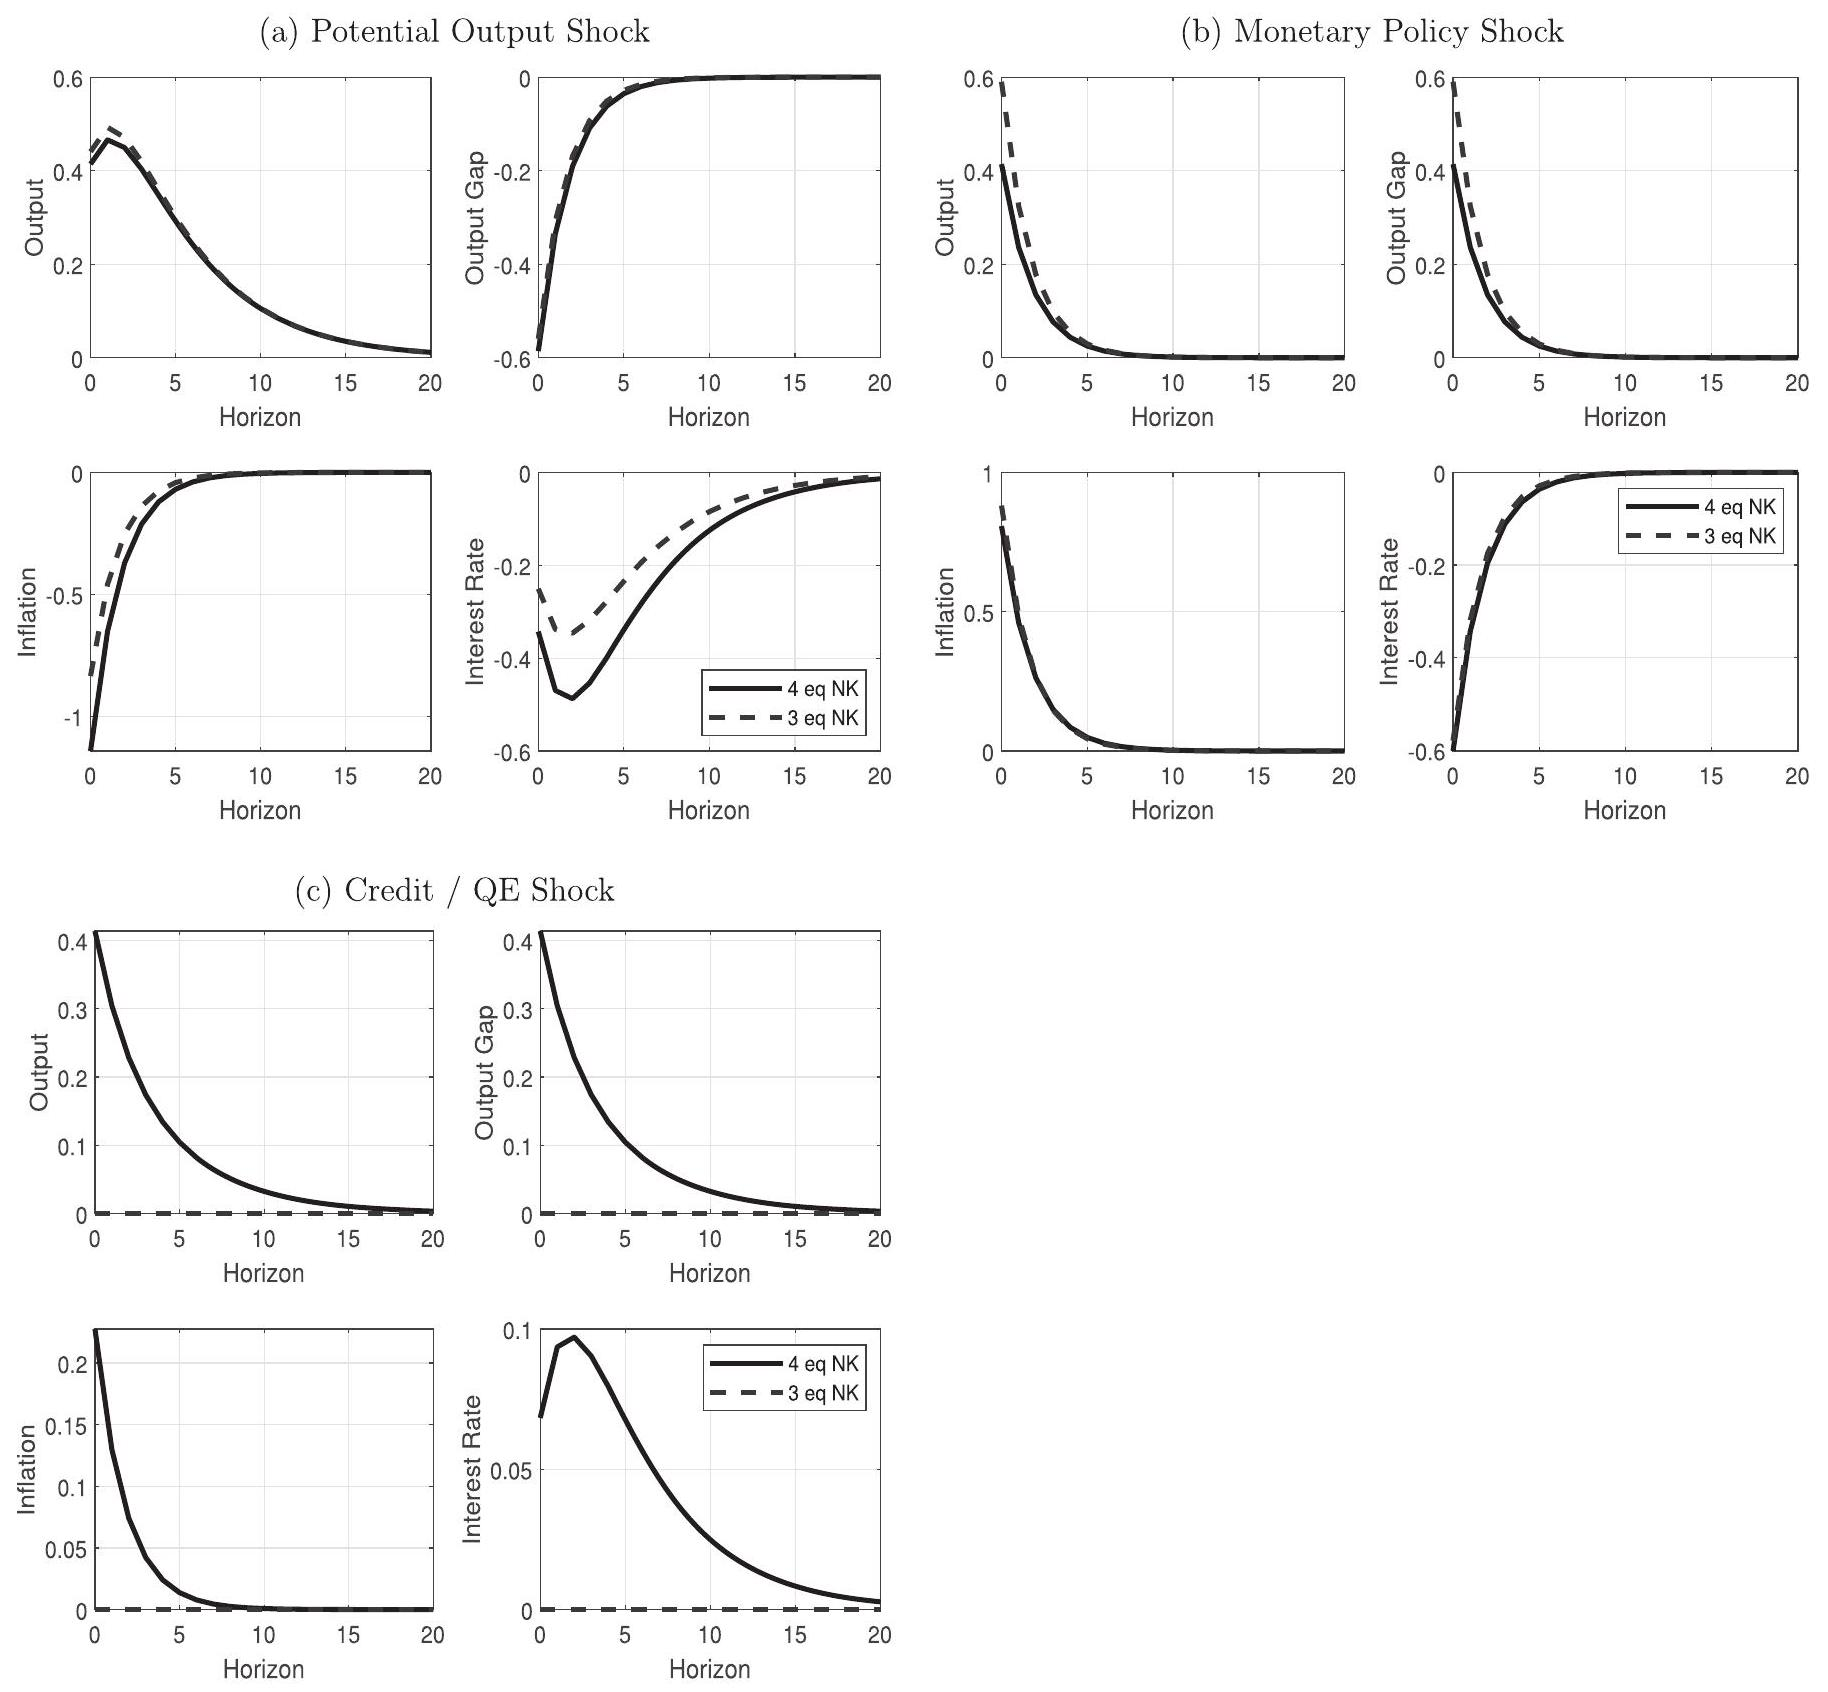
\includegraphics[max width=\textwidth, center]{2024_12_20_098a9c078f922ab7e4b1g-07}\\
(a) IRFs to a 1 percentage point shock to potential output. (b) IRFs to a monetary policy shock. (c) IRFs to a credit/QE shock. Responses of output and the output gap are expressed in percentage points. Responses of inflation and the interest rate are expressed in annualized percentage points. Solid lines shows responses in our four-equation model. Dashed lines are responses in the textbook three-equation model.\\
are standard. The autoregressive parameters in the exogenous processes are all set to 0.8 .

Figure 1 displays impulse responses to shocks in our model. Panel a considers a $1 \%$ positive shock to potential output. ${ }^{5}$ The solid lines are responses in our baseline four

\footnotetext{${ }^{5}$ As written, the linearized model presented in section IIA writes the exogenous process in terms of the natural rate of interest. As shown in online appendix $B$, there is a mapping between the natural rate of interest and potential output. When comparing the four-equation to the three-equation model, the mapping between the natural rate of interest and potential output is not
}
equation model, whereas the dashed lines depict responses in the conventional three-equation model (i.e., our model imposing $z=0$ ). These responses are familiar and do not differ much in our model compared to the more standard threeequation model. Output increases but by less than potential, resulting in a negative output gap. This puts downward pressure on inflation, which is met with policy accommodation

\footnotetext{identical due to the presence of $z$ in the four-equation model. The comparison is more natural for an equal-sized shock to potential output rather than the natural rate of interest.
}
with the short-term interest rate declining. Relative to threeequation model, output reacts slightly less on impact in our model, though this difference is not large.

Figure 1 b plots impulse responses to a conventional monetary policy shock. The size and sign of the shock are chosen to generate the same impact response of output to the potential output shock in the four-equation model. Output (and hence the output gap) rises on impact before reverting to its preshock value. Inflation rises and follows a similar dynamic path as output. As in the case of the potential output shock, there is little meaningful difference in the responses of variables in our four-equation model relative to the baseline three-equation model.

Panel c plots impulse responses to a credit $\left(\theta_{t}\right)$ or $\mathrm{QE}\left(q e_{t}\right)$ shock. Because these differ only according to scale in the linear system $\left(\bar{b}^{F I} \neq \bar{b}^{c b}\right)$, because we have assumed equal AR parameters (0.8), and because the shock sizes are normalized to produce the same impact response of output, the IRFs of endogenous variables to a credit or QE shock are identical. We therefore show only one set of impulse responses.

Unlike responses to the other shocks, in panel c, there is a meaningful difference between the four-equation model and the three-equation model. In the three-equation model, both shocks are irrelevant for the dynamics of endogenous variables. In our four-equation model, an increase in leverage (equivalently a central bank purchase of long bonds) is expansionary for output. In the current calibration, such an expansion also results in an increase in inflation and a resulting increase in the short-term interest rate. That financial shocks have economic effects in line with the traditional understanding of an aggregate demand shock and the fact that there is scope for QE policies represents a key advancement in our four-equation model relative to the standard threeequation model. These properties are critical for understanding the post-crisis economy.

\section*{D. Discussion}
It is fairly standard in macromodels to include reducedform credit shocks as residuals in the IS equation (Smets \& Wouters, 2007). Our structural four-equation model has this feature as well. But in our model, QE and credit shocks also appear as residuals in the Phillips curve, which leads to a breakdown in the divine coincidence and results in potentially important policy trade-offs.

Why do credit shocks appear as an endogenous cost-push wedge in the Phillips curve? Our model's Phillips curve written in terms of marginal cost is the same as in the standard three-equation model,

\begin{equation*}
\pi_{t}=\gamma \widehat{p}_{m, t}+\beta \mathbb{E}_{t} \pi_{t+1}, \tag{38}
\end{equation*}

where $\widehat{p}_{m, t}$ is real marginal cost linearized about the steady state, which is in turn equal to the log difference between the real wage and the marginal product of labor. (See the derivations in online appendix B.)

Holding the aggregate level of output fixed, favorable credit conditions reallocate resources from the parent (the saver) to the child (the borrower). In our model, the parent supplies labor, similar to many other models of financial frictions where workers save and supply variable labor while entrepreneurs borrow and either do not supply labor or do so inelastically (Carlstrom \& Fuerst, 1997). The reallocation of resources when credit conditions are favorable therefore induces a negative wealth effect for the parent that puts downward pressure on the wage, and hence real marginal cost, for a given level of output. This manifests itself as the endogenous cost-push term in the Phillips curve relation written in terms of the output gap.

The credit/QE shocks appearing as an endogenous costpush wedge in the Phillips curve gives rise to an important implication of our model. In our model, a QE shock is less inflationary than a conventional monetary policy rate cut. This finding is in line with the results in the richer model of Sims and $\mathrm{Wu}(2021,2020 b)$ and empirically consistent with the lack of inflationary pressures from the expansive QE operations in the United States and other parts of the world in the wake of the Great Recession. The $q e_{t}$ term enters in both the IS, equation (1), and Phillips curves, equation (2). In particular, $q e_{t}$ enters with a positive sign in the IS relationship, and hence serves as a positive demand shock, but with a negative sign in the Phillips curve. Both of these channels make QE expansionary for output but have competing effects on inflation. As parameterized, an expansionary QE shock in our model is nevertheless inflationary, albeit less so than a conventional monetary policy shock. There also exist parameterizations in which an expansionary QE shock can be deflationary.

Another important difference between a QE shock and a conventional policy shock in our model concerns how each affects the yield curve. Though a long-term interest rate does not appear in the baseline four-equation model in section IIA, one is operating in the background in an alternative representation of the IS curve (see online appendix B):

\begin{equation*}
y_{t}=\mathbb{E}_{t} y_{t+1}-\frac{1}{\sigma}\left(r_{t}^{s}-\mathbb{E}_{t} \pi_{t+1}\right)-\frac{z}{\sigma}\left(\mathbb{E}_{t} r_{t+1}^{b}-r_{t}^{s}\right) . \tag{39}
\end{equation*}

$\mathbb{E}_{t} r_{t+1}^{b}$ is the expected return on the long bond in the model. Hence, the last term in equation (39) can be interpreted as an excess return of the long bond over the short-term rate.

A conventional expansionary monetary policy shock results in a steepening of the yield curve (i.e., an increase in the long rate relative to the short rate). In contrast, a stimulative QE shock results in a flattening of the yield curve. QE works by freeing up space on the FI's balance sheet to purchase long bonds, thereby pushing the price of these bonds higher and the yield lower. There is no direct effect on the short-term rate except through the policy rule. As calibrated, the short rate actually rises modestly (due to the slightly inflationary nature of a QE shock under the current calibration). Impulse responses of the long-short spread to both a conventional policy shock and a QE shock are depicted in figure 2.

Figure 2.-Response of Excess Return of Long Bond to Monetary and QE Shocks\\
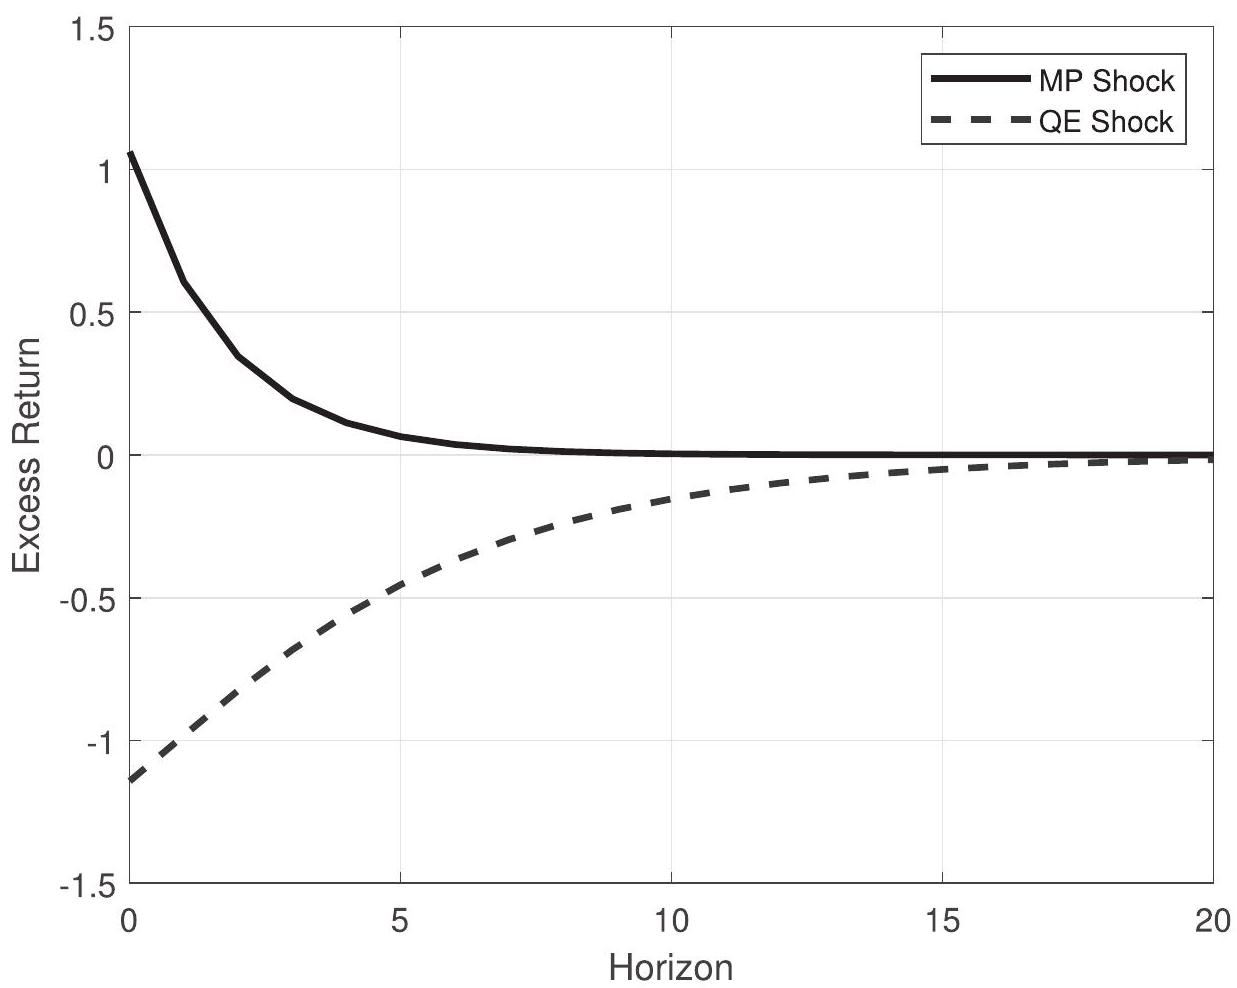
\includegraphics[max width=\textwidth, center]{2024_12_20_098a9c078f922ab7e4b1g-09}

This figures plots the responses of the annualized excess return, $\mathbb{E}_{t} r_{t+1}^{b}-r_{t}^{s}$, inferred from equation (39), to a conventional monetary policy shock (solid line), and a QE shock (dashed line). The shocks are normalized so as to generate the same impact increase in output as in figure 1.

\section*{III. Optimal Monetary Policy}
In this section, we explore the design of optimal monetary policy in the context of our four-equation NK model. Credit shocks generate an endogenous cost-push term in the Phillips curve, so they lead to a nontrivial trade-off for a central bank wishing to solely implement policy via adjustment of the short-term interest rate. As such, heretofore unconventional policies like quantitative easing ought to be used even when the short rate is unconstrained by the ZLB. Further, quantitative easing policies can be a useful (albeit imperfect) substitute for conventional policy when the short-term rate is constrained by the ZLB.

Given policymakers' emphasis on the so-called dual mandate, we focus on a policy-relevant quadratic loss function in inflation and the output gap:

\begin{equation*}
\mathbb{L}=\mu x_{t}^{2}+\pi_{t}^{2} . \tag{40}
\end{equation*}

$\mu \geq 0$ is the relative weight attached to fluctuations in the output gap. An expression like equation (40) can be motivated as the microfounded welfare criterion for a central bank in the standard three-equation NK model under certain assumptions. ${ }^{6}$ The central bank's welfare objective is a

\footnotetext{${ }^{6}$ In particular, in the benchmark three-equation model equation (40) would be the microfounded loss function when a Pigouvian tax is in place to undo the steady-state distortion associated with monopolistic competition (see
}
present discounted value of the period loss function given in equation (40). For the remainder of this section, we consider optimal policy under discretion, and so focus only on the period loss function.

\section*{A. Unconstrained Optimal Discretionary Policy}
We begin by studying optimal monetary policy when both policy instruments are available. We start with an impossibility result spelled out formally in theorem 1 :

Theorem 1. It is not possible to completely stabilize both inflation and the output gap with the adjustment of a single policy instrument when both credit and natural rate shocks are present.

Proof. See online appendix G.1.

Woodford (2003). The optimal weight on the output gap would satisfy $\mu=\frac{\gamma \zeta}{\epsilon}$, where $\gamma \zeta$ is the slope of the Phillips curve and $\epsilon$ is the elasticity of substitution across varieties of retail goods. For conventional calibrations, this weight would be quite low.

In our four-equation model, a fully microfounded loss function would be more complicated due to the two types of households and would depend on arbitrary welfare weights on each. We instead choose to focus on a policyrelevant loss function like equation (40) and consider a variety of different values of $\mu$. One can motivate targeting $y_{t}^{*}$ as the appropriate output level in a version of a social planner's problem where the planner wishes to completely smooth the consumption of the child household. See online appendix D.

This result can be viewed as a straightforward application of Tinbergen (1952). But the result is particularly interesting and useful in our setting because the credit shock breaks the divine coincidence (Blanchard \& Galí, 2007), in which case, one policy instrument is sufficient to hit both targets. In our model, it is not possible to simultaneously stabilize inflation and the output gap with only the short-term policy rate.

Given the impossibility result of theorem 1 , the central bank should use both the short-term rate and its long bond portfolio as policy instruments. Each period, the central bank minimizes its loss function in equation (40) with respect to the two policy instruments ( $r_{t}^{s}$ and $q e_{t}$ ) subject to the IS and Phillips curves in equations (1) and (2). As shown formally in online appendix G.1, the optimal solution features $\pi_{t}=$ $x_{t}=0$ (i.e., the central bank hits both of its targets).

In equilibrium, simultaneously hitting both targets leads to the following optimal paths of the central bank's instruments:

Proposition 1. With both instruments available, the central bank achieves $\pi_{t}=x_{t}=0$, and the equilibrium paths for the policy instruments are $r_{t}^{s}=r_{t}^{*}$ and $q e_{t}=-\frac{\bar{b}^{F I}}{\bar{b}^{c b}} \theta_{t}$.

The proof of proposition 1 is simple. From the Phillips curve, inflation and the output gap always equaling zero implies that $q e_{t}=-\frac{\bar{b}^{F I}}{\bar{b}^{c b}} \theta_{t}$. Then, from the IS equation, we must have $r_{t}^{s}=r_{t}^{*}$. The novel implication of proposition 1 is that QE-type policies in principle ought to always be used as long as there are credit shocks, not only when the short-term policy rate is constrained by the ZLB.

\section*{B. Optimal QE at the ZLB}
Although QE-type policies should always be used to offset credit market disturbances in our model, they became popular only when short-term interest rates were pushed to the ZLB in the wake of the financial crisis and ensuing Great Recession. In this section, we study how QE policies might be used to mitigate the consequences of a binding ZLB.

We approximate the effects of a binding ZLB in our linearized model following Eggertsson and Woodford (2003) and Christiano, Eichenbaum, and Rebelo (2011). Suppose that a central bank has been following the jointly optimal policy described in proposition 1. But then in period $t$, suppose the natural rate of interest falls below 0 , so that $r_{t}^{s}=0$. Suppose that it will stay there in each subsequent period with probability $\alpha \in[0,1)$, where this probability is invariant over time. The expected duration of the ZLB is therefore $1 /(1-\alpha)$. This means that interest rate policy can be characterized as follows:\\
\begin{align*}
r_{t}^{s} & =0  \tag{41}\\
\mathbb{E}_{t} r_{t+1}^{s} & =0 \text { with probability } \alpha . \tag{42}
\end{align*}

Faced with a ZLB, the central bank will pick $q e_{t}$ to minimize its loss function, but it is unable to pick the policy rate.

The optimal choice of $q e_{t}$ leads to the following lean-against-the-wind-condition,

\begin{equation*}
\pi_{t}=-\frac{\mu(1-z)}{\gamma \zeta(1-z)-\gamma \sigma} x_{t} . \tag{43}
\end{equation*}

Proposition 2 describes the evolution of targets and instruments while the ZLB is binding.\\
Proposition 2. When the short rate is constrained by the $Z L B$, which will continue to bind in the next period with probability $\alpha$, with QE being the only viable policy instrument, the optimal targeting rule is characterized by equation (43). In equilibrium, the paths for inflation, output gap, and QE are\\
\begin{align*}
\pi_{t} & =\omega_{1} r_{t}^{*}  \tag{44}\\
x_{t} & =\omega_{1} \omega_{2} r_{t}^{*}  \tag{45}\\
q e_{t} & =\tau r_{t}^{*}-\frac{\bar{b}^{F I}}{\bar{b}^{c b}} \theta_{t} \tag{46}
\end{align*}\\
where\\
\begin{align*}
\omega_{1} & =\frac{\gamma(1-z)}{\binom{\gamma \sigma\left(1-\alpha \rho_{f}\right) \omega_{2}-\alpha \gamma \rho_{f}(1-z)}{+(1-z)\left(1-\alpha \rho_{f}\right)\left(1-\gamma \zeta \omega_{2}-\alpha \beta \rho_{f}\right)}}  \tag{47}\\
\omega_{2} & =-\frac{\gamma \zeta(1-z)-\gamma \sigma}{\mu(1-z)}  \tag{48}\\
\tau & =-\frac{\left(1-\gamma \zeta \omega_{2}-\alpha \beta \rho_{f}\right)(1-z)}{z \gamma \sigma \bar{b}^{c b}} \omega_{1} \tag{49}
\end{align*}

Proof. See online appendix G.2.\\
An important and novel implication of proposition 2 is that the ZLB need not pose a problem for credit shocks; inflation and the gap can be completely stabilized when only QE is available, with the QE portfolio adjusting to credit shocks exactly as it would absent the ZLB.

More important, we use the results from proposition 2 to investigate the extent to which QE can serve as an effective substitute for conventional monetary policy during periods in which the short-term interest rate is constrained by 0 . This was the original motivation for the use of QE in countries like Japan and the United States when policy rates moved to the ZLB.

We restrict attention to values of $\alpha$ where $\omega_{1}>0$, so that reductions in the natural rate of interest cause inflation and the gap to decline when the ZLB binds. ${ }^{7}$ In this region, $\tau<0$,

\footnotetext{${ }^{7}$ As noted in Carlstrom, Fuerst, and Paustian (2014), that for sufficiently large $\alpha$, the sign of $\omega_{1}$ can flip from positive to negative. Where this perverse sign flip occurs depends on the values of other parameters, such as the slope of the Phillips curve, $\gamma \zeta$. We restrict attention to values of $\alpha$ consistent with $\omega_{1}$ being positive. For our parameterization, the sign flip occurs at an $\alpha$ consistent with an expected ZLB duration of thirteen or more quarters. An alternative experiment would be to make the duration of the ZLB
}Figure 3.-IRFs to Natural Rate Shock at the ZLB, Optimal QE, DifFerent $\mu$\\
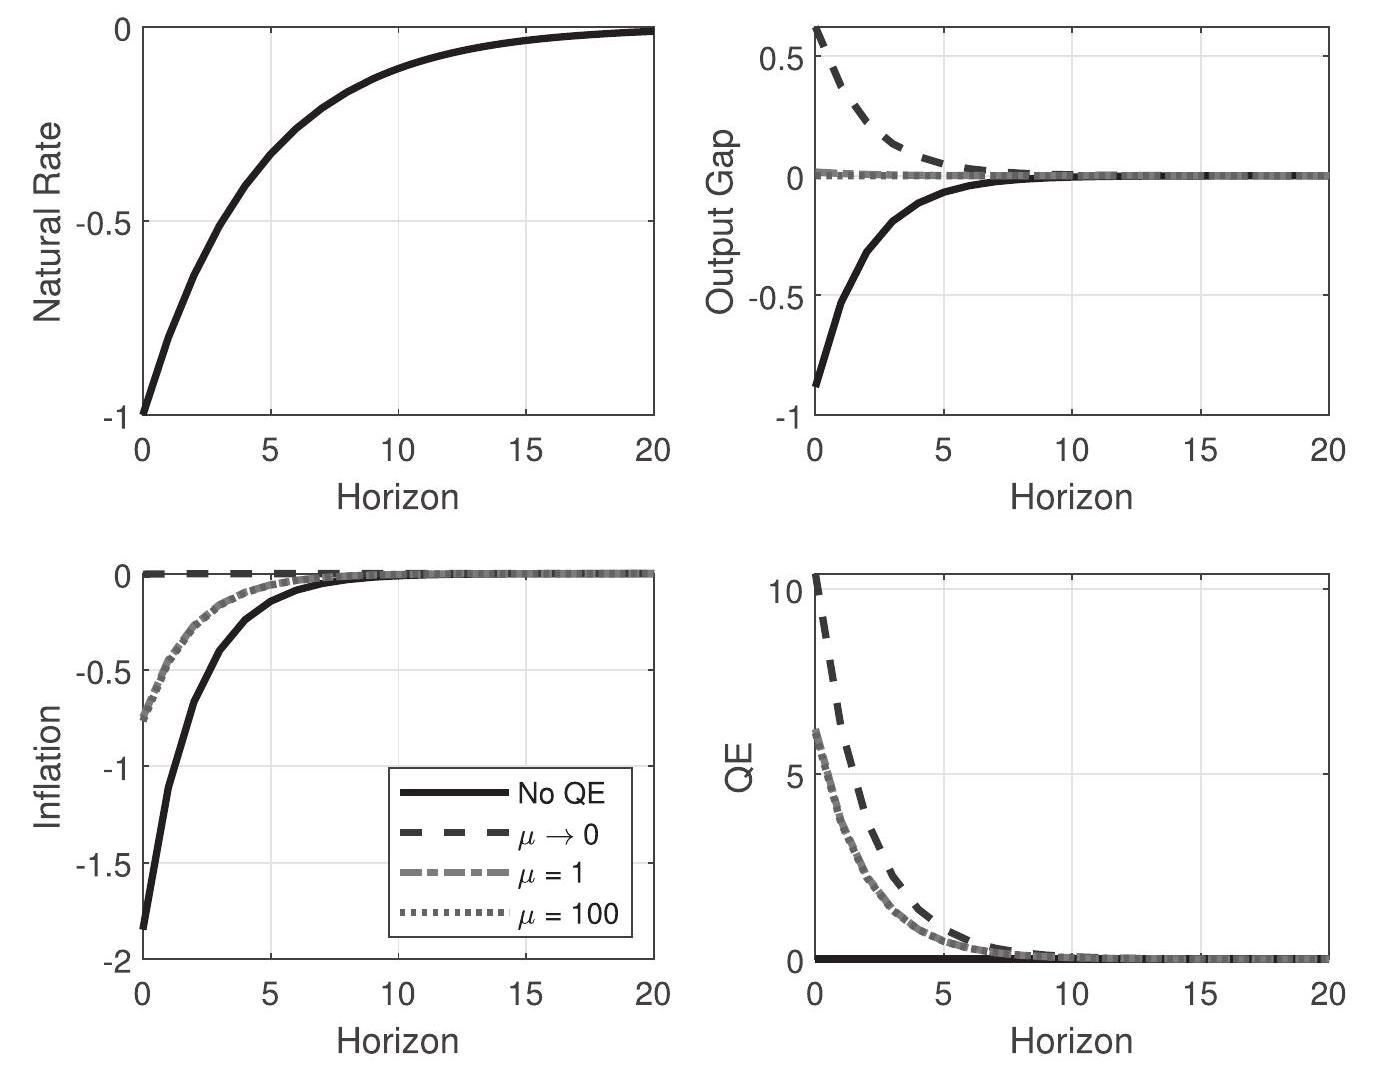
\includegraphics[max width=\textwidth, center]{2024_12_20_098a9c078f922ab7e4b1g-11}

Solid lines: IRFs to a 100 basis point shock to the natural rate of interest in the four-equation model when the short-term interest rate is constrained by the ZLB for $1 /(1-\alpha)$ periods in expectation, where $\alpha=3 / 4$, and there is no endogenous QE to the natural rate shock. The dashed lines plot responses with the optimally chosen $\tau$ for different welfare weights on the output gap, $\mu$. The output gap is expressed in percentage points, while the responses of inflation and the short-term interest rate are in annualized percentage points.\\
which means that the central bank provides a positive stimulus in the form of bond purchases when the natural rate of interest declines. We show in online appendix H that $\tau$ is increasing in $\alpha$ in this region. In other words, QE optimally reacts more aggressively to a natural rate shock the longer is the expected duration of the ZLB.

Figure 3 shows responses to a contractionary natural rate shock when the ZLB binds. Solid lines depict responses when QE is unavailable. The ZLB binds for four quarters in expectation, with $\alpha=3 / 4$. With neither QE nor the policy rate available, the output gap and inflation both decline significantly in response to a negative natural rate shock. A binding ZLB entails significant welfare losses.

The colored nonsolid lines in figure 3 plot responses when the ZLB binds but QE is optimally implemented. We consider different values of $\mu$, the relative weight on fluctuations in the output gap. When the central bank places no weight on the output gap (i.e., $\mu \rightarrow 0$ ), inflation is completely stabilized, the output gap increases (rather than decreases), and the central bank increases the size of its long bond portfolio by a sizable amount. When virtually all weight is placed on the gap ( $\mu=100$ ), in contrast, inflation declines, although

\footnotetext{deterministic rather than stochastic. There would be no sign flip at some sufficiently long duration, but the analytic expression for $\omega_{1}$ would be significantly more complicated.
}
much less than the no-QE benchmark, the gap is completely stabilized, and the increase in the value of the long bond portfolio is much more modest compared to the $\mu \rightarrow 0$ case. The case of equal weight on inflation and the gap is virtually indistinguishable from the case of nearly all weight being on the gap in the loss function.

The results described in figure 3 suggest that quantitative easing can be an effective, albeit imperfect, substitute for conventional policy in response to natural rate shocks at the ZLB. For example, in the case of equal relative weights ( $\mu=$ 1), the output gap essentially does not react to the natural rate shock and inflation falls by about two-thirds of a percent given optimal QE policy. In comparison, with no endogenous QE at the ZLB , the output gap would decline by nearly a full percentage point, and inflation would fall by about three times as much. Endogenous QE therefore entails a sizable welfare improvement over doing nothing at the ZLB. This will be true regardless of the value of $\mu$.

The response of the central bank's bond portfolio to a natural rate shock is always opposite the shock, but the magnitude depends on the relative weight the central bank places on the output gap in its loss function, $\mu$. For a central bank concerned solely with stabilizing inflation, it is optimal to adjust the long bond portfolio quite strongly in response to natural rate shocks. For a central bank more concerned with gap stabilization, the optimal QE response remains sizable but is\\
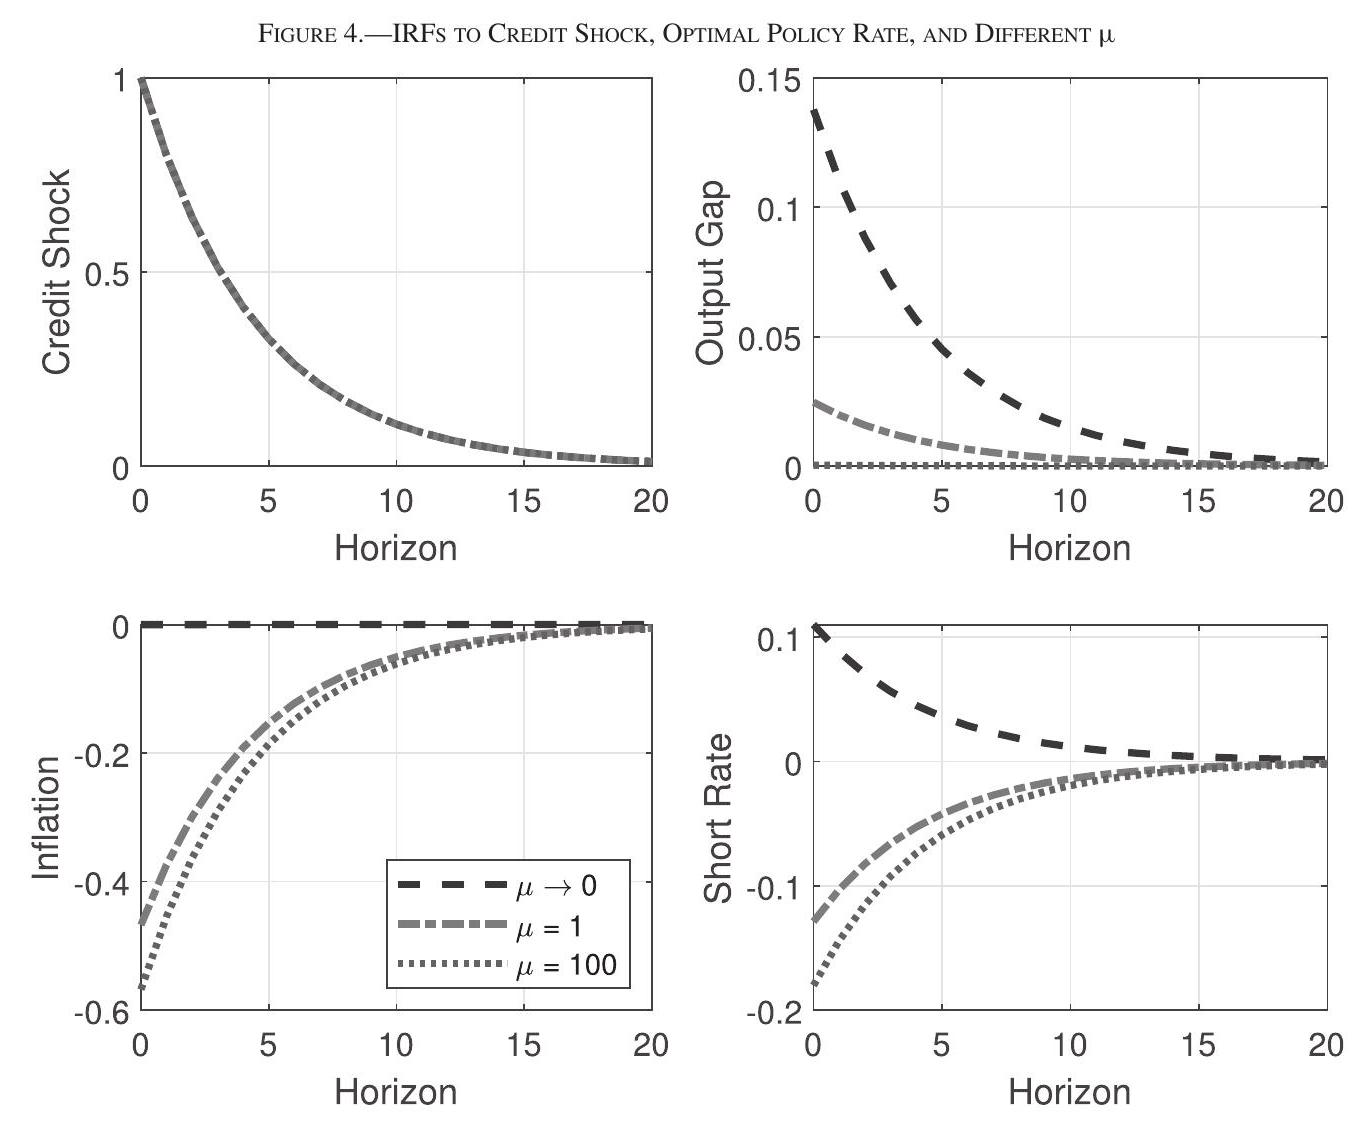
\includegraphics[max width=\textwidth, center]{2024_12_20_098a9c078f922ab7e4b1g-12}

This figure plots IRFs to a 1 percentage point credit shock in the four-equation model. $q e_{t}=0$, and the interest rate is set according to the optimality condition described in proposition 3 . The output gap is expressed in percentage points, while the responses of inflation and the short-term interest rate are in annualized percentage points.\\
nevertheless quite a bit smaller than for values of $\mu$ close to zero. See online appendix H for a figure plotting the optimal $\tau$ as a function of $\mu$.

\section*{C. Optimal Policy without QE}
Next, consider an operating framework similar to the one prevailing in the United States prior to the Great Recession in which the central bank uses the short-term interest rate as its sole policy instrument. The ZLB does not bind. This section studies the optimal adjustment of the short-term rate in this scenario.

As shown in online appendix G.3, the optimal choice of the policy rate satisfies

\begin{equation*}
\pi_{t}=-\frac{\mu}{\gamma \zeta} x_{t} \tag{50}
\end{equation*}

Note that equation (50) is the same as the lean-against-the-wind-condition for the policy rate for optimal policy under discretion as in the canonical three-equation model. With equation (50) characterizing optimal policy, the equilibrium paths of endogenous variables are given by:\\
Proposition 3. With the short rate being the only policy instrument, the optimal targeting rule is characterized by equation (50). In equilibrium, the paths for inflation, the output\\
gap, and the policy rate are\\
\begin{align*}
\pi_{t} & =\varphi \theta_{t}  \tag{51}\\
x_{t} & =-\frac{\gamma \zeta}{\mu} \varphi \theta_{t},  \tag{52}\\
r_{t}^{s} & =r_{t}^{*}+\eta \theta_{t}, \tag{53}
\end{align*}\\
where\\
\begin{align*}
\varphi & =-\frac{\mu}{\gamma^{2} \zeta^{2}+\mu\left(1-\beta \rho_{\theta}\right)} \frac{z \gamma \sigma}{1-z} \bar{b}^{F I}  \tag{54}\\
\eta & =\rho_{\theta} \varphi+\frac{\sigma\left(1-\rho_{\theta}\right)}{1-z} \frac{\gamma \zeta}{\mu} \varphi+\frac{\left(1-\rho_{\theta}\right) \sigma z \bar{b}^{F I}}{1-z} \tag{55}
\end{align*}

\section*{Proof. See online appendix G.3.}
The optimal policy described in proposition 3 completely stabilizes the output gap and inflation in response to natural rate shocks. This is not true conditional on credit shocks. Figure 4 plots the responses of the output gap and inflation to a credit shock for different values of $\mu$, taking our baseline calibration of other parameters.

When there is no weight placed on the output gap, shown with the dashed lines corresponding to $\mu \rightarrow 0$, the central\\
bank raises the short-term interest rate in response to a positive credit shock (i.e., $\eta>0$ ). This completely stabilizes inflation but results in a sizable increase in the output gap. In contrast, if the relative weight on the output gap is large ( $\mu=100$, shown in the dotted lines), the central bank optimally cuts the policy rate in response to the credit shock (i.e., $\eta<0$ ). This stabilizes the output gap but results in a significant decline in inflation. For equal weights on the output gap and inflation ( $\mu=1$, depicted via dash-dotted lines), the policy rate decreases slightly, but the output gap rises and the inflation rate falls.

An interesting result from figure 4 is that the sign of the optimal policy rate response to a credit shock depends on the relative weight placed on the output gap. A central bank mostly concerned with stabilizing output ought to cut the policy rate in the face of a positive credit shock, whereas it should raise the policy rate if it is mostly concerned with stabilizing inflation. In online appendix $H$, we plot $\eta$ as a function of $\mu$. Consistent with what is observed in figure $4, \eta$ is positive when $\mu$ is very small and turns negative as $\mu$ gets bigger, crossing 0 at around $\mu=1$. For central banks facing a dual mandate, this trade-off between stabilizing inflation or the output gap can be eliminated if they can deploy QE.

\section*{IV. Implementable Policy Rules}
In section III, we explored optimal monetary policy under discretion. We derived first-order conditions for a central bank facing a standard welfare function. These first-order conditions are optimal targeting rules that imply paths of the short-term policy rate and the central bank's long bond portfolio. With both instruments available, it is possible to completely stabilize both inflation and the gap. In equilibrium, the policy rate moves one-for-one with the natural rate of interest, and the long bond portfolio moves opposite credit shocks.

While optimal targeting rules have a long tradition in the monetary policy literature, there is also significant interest in the design of instrument rules where instruments react to fluctuations in endogenous variables. In this section, we therefore consider the optimal design of simple and implementable rules for both the short-term policy rate and the central bank's long bond holdings (Schmitt-Grohe \& Uribe, 2007). We assume that the short-term policy rate obeys a standard Taylor rule, equation (34). We further allow for the central bank's long bond portfolio to obey a similar Taylor-type rule that reacts to inflation and the output gap:

\begin{equation*}
q e_{t}=\rho_{q} q e_{t-1}-\left(1-\rho_{q}\right)\left[\lambda_{\pi} \pi_{t}+\lambda_{x} x_{t}\right]+s_{q} \varepsilon_{q, t} . \tag{56}
\end{equation*}

In postulating equation (56), which we refer to as a "QE rule," we assume that $\lambda_{\pi} \geq 0$ and $\lambda_{x} \geq 0$. The negative sign in front reflects the fact that, a priori, we think that the central bank would want to move its bond holdings opposite the direction of how it would adjust the policy rate in reaction to movements in both inflation and the output gap.

\section*{A. Determinacy}
An important requirement for instrument rules is that they deliver a determinate rational expectations equilibrium. As shown in online appendix C , if there is no endogenous component to the QE rule (i.e., $\lambda_{\pi}=\lambda_{x}=0$ ), then the restrictions necessary for determinacy on the coefficients of the Taylor rule for the policy rate are the same as in the standard three-equation New Keynesian model. This will not necessarily be the case when the central bank's bond holdings react to inflation and the output gap. In this section, we consider how endogenous reactions in the QE rule affect equilibrium determinacy.

Let $\mathbf{z}_{t}=\left[\begin{array}{llll}\pi_{t} & x_{t} & r_{t-1}^{s} & q e_{t-1}\end{array}\right]^{\prime}$ be the vector of linearized endogenous variables. ${ }^{8}$ The system evolves according to

\begin{equation*}
\mathbb{E}_{t} \mathbf{z}_{t+1}=\mathbf{A} \mathbf{z}_{t} \tag{57}
\end{equation*}

With two predetermined states, a unique rational expectations equilibrium requires that there be exactly two unstable eigenvalues in $\mathbf{A}$.

Because of the additional complexity of a fourth endogenous variable, we only numerically characterize the portion of the parameter space necessary for determinacy. We fix most parameter values at those listed in table 1 . We then consider different values of $\lambda_{\pi}$ and $\lambda_{x}$ and search for the minimum combination of $\phi_{\pi}$ and $\phi_{x}$ needed to generate determinacy, conditional on those values of $\lambda_{\pi}$ and $\lambda_{x} .{ }^{9}$

Consider first the different values of $\lambda_{\pi}$, fixing $\lambda_{x}=0$. We consider values of $\lambda_{\pi}$ of $0,1.5,5$, and 15 . Results are shown graphically in figure 5 a . When $\lambda_{\pi}=\lambda_{x}=0$, we have the familiar result (shown in the solid line) that when $\phi_{x}=0$, the central bank must respond at least one-to-one with inflation in the interest rate rule. As $\phi_{x}$ rises, the required value of $\phi_{\pi}$ falls, but determinacy is mostly governed by the response to inflation. When $\lambda_{\pi}>0$, so long as $\phi_{x}=0$, it remains the case that the interest rate rule must react more than one-toone to inflation for determinacy. There is an interaction effect between $\lambda_{\pi}$ and $\phi_{x}$, however. For modestly positive values of $\lambda_{\pi}$, as $\phi_{x}$ gets bigger, the requisite coefficient on inflation in the interest rate rule for equilibrium determinacy gets larger instead of smaller. This effect is more noticeable the bigger is $\lambda_{\pi}$ and seems quantitatively relevant. In particular, suppose that $\phi_{x}=1$. When $\lambda_{\pi}=\lambda_{x}=0$, the requisite value of $\phi_{\pi}$ is slightly less than 1 . But when $\lambda_{\pi}=5$, the required coefficient on inflation in the interest rate rule is about 1.3. When $\lambda_{\pi}=$ 15 , the necessary value of $\phi_{\pi}$ jumps to more than 2 .

Our intuition for the above results is as follows. For a determinate equilibrium, the policy rate must react more than one-for-one to a permanent change in the inflation rate. If the Taylor rule for the policy rate does not react to the output gap, we have the standard Taylor principal condition that $\phi_{\pi}>1$, regardless of whether the central bank's long bond portfolio

\footnotetext{${ }^{8}$ See online appendix C for more details.\\
${ }^{9}$ For these exercises, we set $\rho_{r}=\rho_{q}=0.8$. Results are very similar for different values of these smoothing parameters.
}Figure 5.—Policy Coefficients For Determinacy\\
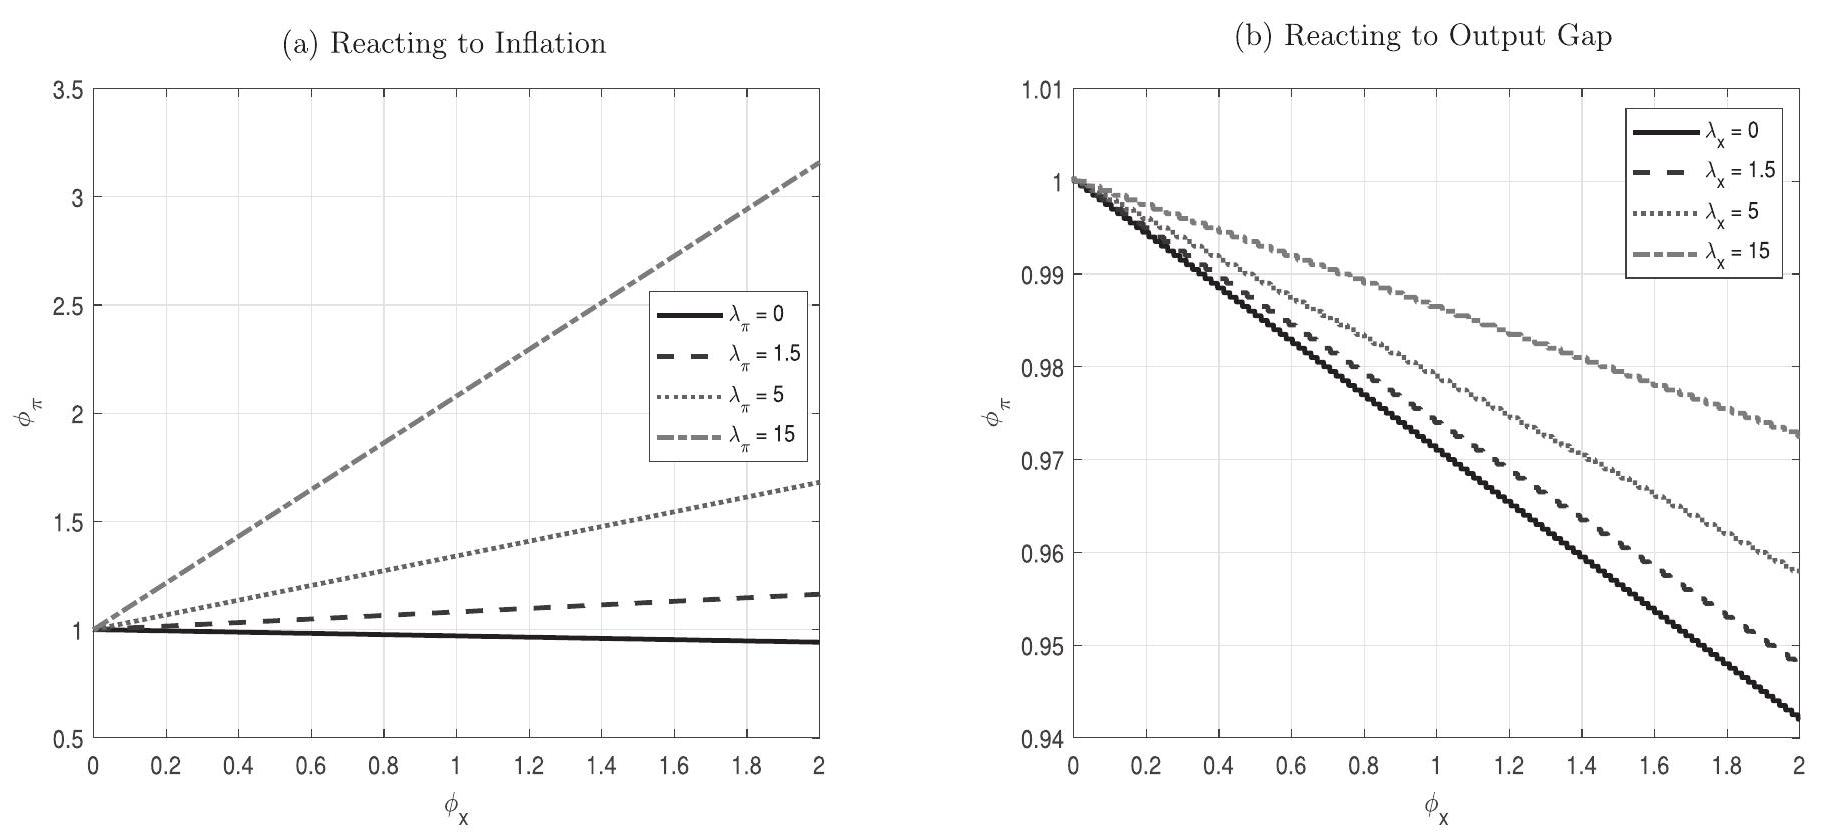
\includegraphics[max width=\textwidth, center]{2024_12_20_098a9c078f922ab7e4b1g-14}\\
(a) The minimum values of $\phi_{\pi}$ and $\phi_{x}$ (the reactions to inflation and the output gap, respectively, in the interest rate rule) necessary for equilibrium determinacy, conditional on different values of $\lambda_{\pi}$ (the reaction to inflation in the QE rule). $\lambda_{x}=0$. The solid line considers the case of $\lambda_{\pi}=0$, the dashed line the case of $\lambda_{\pi}=1.5$, the dotted line in the case of $\lambda_{\pi}=5$, and the dash-dotted line the case of $\lambda_{\pi}=15$. Values of $\phi_{\pi}$ above each line generate a unique rational expectations equilibrium. (b) Plots of the minimum values of $\phi_{\pi}$ and $\phi_{x}$ (the reactions to inflation and the output gap, respectively, in the interest rate rule) necessary for equilibrium determinacy, conditional on different values of $\lambda_{x}$ (the reaction to the output gap in the QE rule). $\lambda_{\pi}=0$. The solid line considers the case of $\lambda_{x}=0$, the dashed line the case of $\lambda_{x}=1.5$, the dotted line the case of $\lambda_{x}=5$, and the dash-dotted line the case of $\lambda_{x}=15$. Values of $\phi_{\pi}$ above each line generate a unique rational expectations equilibrium.\\
reacts to inflation. When $\phi_{x}>0$ and QE reacts to inflation, in contrast, the cutoff value of $\phi_{\pi}$ is bigger than 1 . When QE reacts negatively to inflation, there exists downward pressure on the output gap, other factors held constant. When the policy rate also reacts positively to the output gap, taken together, an active QE rule reduces the overall sensitivity of the policy rate to inflation for a given $\phi_{\pi}$. The bigger the reaction of QE to inflation and the larger the reaction of the policy rate to the gap, the more aggressive must be the direct response to inflation in the Taylor rule.

Consider next different values of $\lambda_{x}$, fixing $\lambda_{\pi}=0$. We again consider values of $\lambda_{x}$ of $0,1.5,5$, and 15 . Results are depicted graphically in figure 5 b. Here the determinacy results are more in line with the standard three-equation model. In particular, responding more strongly to the output gap in the interest rate rule permits a smaller reaction to inflation for any value of $\lambda_{x}$. The required coefficient on inflation in the interest rate rule, $\phi_{\pi}$, is larger for each value of $\phi_{x}$ the bigger is the reaction to the gap in the QE rule, $\lambda_{x}$. But the differences in the necessary values of $\phi_{\pi}$ for each $\phi_{x}$ when $\lambda_{x}$ gets larger are quite small.

There are two noteworthy conclusions from these exercises. First, a QE rule that reacts aggressively to endogenous variables like inflation and the output gap does not make equilibrium determinacy more likely in our model. In fact, it makes it less likely: larger values of $\lambda_{\pi}$ or $\lambda_{x}$ reduce, rather than increase, the set of coefficients in the interest rate rule that yield a unique rational expectations equilibrium. Second, for the purposes of guaranteeing a determinate equilibrium,\\
reacting to inflation in the QE rule seems more problematic than reacting to the output gap. QE responding to the output gap, but not inflation, hardly has any effect on the set of coefficients in the interest rate rule that result in determinacy. The QE rule reacting to inflation, in contrast, both introduces a trade-off between reacting to the output gap and inflation in the interest rate rule, and significantly increases the required coefficient on inflation in that rule. ${ }^{10}$ In practice, central banks have implemented QE during episodes of low interest rates and inflation and have primarily used it to target real variables. In this case, indeterminacy is less likely to be an issue.

\section*{B. Optimal Implementable Rules}
In this section, we consider optimal implementable policy rules, of the forms (34) for the interest rate rule and (56) for the QE rule. There are six policy parameters: $\rho_{r}, \phi_{\pi}$, and $\phi_{x}$ for the interest rate rule, and $\rho_{q}, \lambda_{\pi}$, and $\lambda_{x}$ for the QE rule. The assumed objective function of a central bank, equation (40), features two targets (inflation and the output gap). Our model structure features two instruments (the shortterm interest rate and the central bank's bond portfolio). With this many parameters and only two targets (inflation and the

\footnotetext{${ }^{10} \mathrm{To}$ be clear, by trade-off we mean that conditional on reacting to inflation in the QE rule, the central bank must react more to inflation in the interest rate rule the more it reacts to the output gap. In contrast, in the threeequation model, no such trade-off exists: responding more to the gap in the interest rate rule necessitates reacting less to inflation.
}
output gap), there may in principle be many configurations of these policy parameters that give rise to desirable outcomes. We focus on one particularly simple and transparent specification: the interest rate rule ought to react strongly to inflation, while the QE rule should react aggressively to the output gap. This both ensures equilibrium determinacy given our results above and also seems to be the relevant case in practice.

For the purposes of the exercises that follow, we set both autoregressive parameters ( $\rho_{r}$ and $\rho_{q}$ ) equal to 0 . Results are qualitatively similar for positive values of the smoothing parameters. We set the coefficient on the output gap in the interest rate rule, $\phi_{x}$, and the coefficient on inflation in the QE rule, $\lambda_{\pi}$, equal to 0 . We then show how both targets and instruments react to exogenous shocks for different values of the coefficient on inflation in the interest rate rule, $\phi_{\pi}$, and the coefficient on the output gap in the QE rule, $\lambda_{x}$.

Figure 6a shows impulse responses to a shock to potential output. Solid lines show the optimal responses discussed in section III. Under the optimal policy, inflation and the output gap are completely stabilized, with the interest rate reacting one-for-one with the natural rate and the central bank's bond portfolio unaffected. The dashed lines show the situation in which the interest rate rule reacts to inflation, with $\phi_{\pi}=1.5$, but bond holdings are constant. Relative to the optimal outcome, the interest rate overreacts, with both inflation and the output gap increasing. The dotted lines consider the case where $\phi_{\pi}=1.5$, but the QE rule reacts to the output gap, with $\lambda_{x}=1.5$. The central bank's bond holdings fall, with the output gap and inflation both increasing less than the case where $\phi_{\pi}=1.5$ and $\lambda_{x}=0$. The dashed dash-dotted lines consider the case where $\phi_{\pi}=\lambda_{x}=5$. This represents a more noticeable improvement, with both inflation and the output gap reacting less to the shock. Lines with plus markers consider the case where $\phi_{\pi}=\lambda_{x}=15$. The output gap and inflation both increase but only slightly. Furthermore, the paths of the interest rate and central bank bond holdings are closer to the optimal paths. As $\phi_{\pi}=\lambda_{x} \rightarrow \infty$, the responses of all variables, both targets and instruments, approach their optimal paths.

Figure 6 b is structured similarly but considers responses to the credit shock, $\theta_{t}$. With the optimal policy, inflation and the output gap are constant, with the central bank's bond holdings falling and the interest rate being constant. When the central bank only reacts using the interest rate, with $\phi_{\pi}=1.5$, and $\lambda_{x}=0$, both inflation and the output gap increase, with the interest rate increasing as a result. As the central bank adjusts its bond portfolio more aggressively to the output gap, these movements are smaller. As in the case of the natural rate shock, as $\phi_{\pi}=\lambda_{x} \rightarrow \infty$, the responses of all variables approach their optimal paths.

In our four-equation model, in equilibrium the optimal discretionary policy results in the interest rate moving one-forone with changes in the exogenous natural rate of interest and the central bank's bond portfolio moving opposite the credit shock. A central bank can closely replicate these paths via

Taylor-type instrument rules for both the interest rate and its bond portfolio. Doing so requires aggressively responding to inflation in the interest rate rule and reacting strongly to the output gap in the QE rule.

\section*{C. Implementable Rules and the ZLB}
In practice, quantitative easing and other forms of unconventional monetary policy have been deployed primarily as antidotes to conventional policy paralysis at the ZLB. In section III, in the context of optimal targeting rules, we examined how QE could be deployed as a useful albeit imperfect substitute for conventional policy at the ZLB. In this section, we proceed similarly, but instead focus on an implementable rule for the central bank's long bond portfolio of the form (56).

We solve the linearized four-equation model using a piecewise linear approximation subject to the constraint that the policy rate be nonnegative. In implementing the ZLB, we follow Guerrieri and Iacoviello (2015). As long as this constraint is not binding, the policy rate obeys equation (34). To implement a binding ZLB, we subject the economy to a sequence of natural rate shocks that force the nonnegativity constraint to bind, in expectation for two years (eight quarters). To compute impulse responses, in the first period that the ZLB binds, we also subject the economy to a small shock to either the natural rate or the credit variable, where the shock is small enough so as to not change the expected length of time the ZLB is binding. We compare how the economy reacts to these shocks when QE is fixed versus when it obeys equation (56).

Figure 6 c plots impulse responses to a potential output shock under three scenarios. The solid lines depict responses when there is no ZLB and the policy rate follows a simple Taylor rule with $\phi_{\pi} \rightarrow \infty$; QE is held fixed. As discussed above, a very large reaction to the inflation rate in the Taylor rule for the policy rate replicates the optimal allocations under discretion. The dashed lines depict responses when the ZLB binds for eight quarters and QE is still unavailable. During the period of the ZLB, $r_{t}^{s}=0$; when the ZLB lifts, it follows the simple rule with a very large reaction to inflation. The binding ZLB results in both the output gap and inflation declining substantially while the ZLB binds; once the ZLB lifts, both return to 0 . The dotted lines consider the case where QE is not fixed; rather, it follows a rule in which it reacts very strongly to the output gap, with $\lambda_{x} \rightarrow \infty$. This results in complete stabilization of the gap, even during the ZLB. Inflation still falls, although not as markedly as when the ZLB binds and QE is unavailable. The central bank's long bond portfolio must react aggressively to the natural rate shock, as depicted in the lower right corner of the figure. Note that the responses in figure 6 c with implementable rules are qualitatively similar to what is shown in figure 3 for optimal targeting rules. ${ }^{11}$

\footnotetext{${ }^{11}$ Note in this exercise that the ZLB lasts for eight periods with certainty, whereas in section III, the ZLB only lasted for four quarters in expectation. Hence, the scales in the two sets of figures are not directly comparable.
}Figure 6.-IRFs with Implementable Rules\\
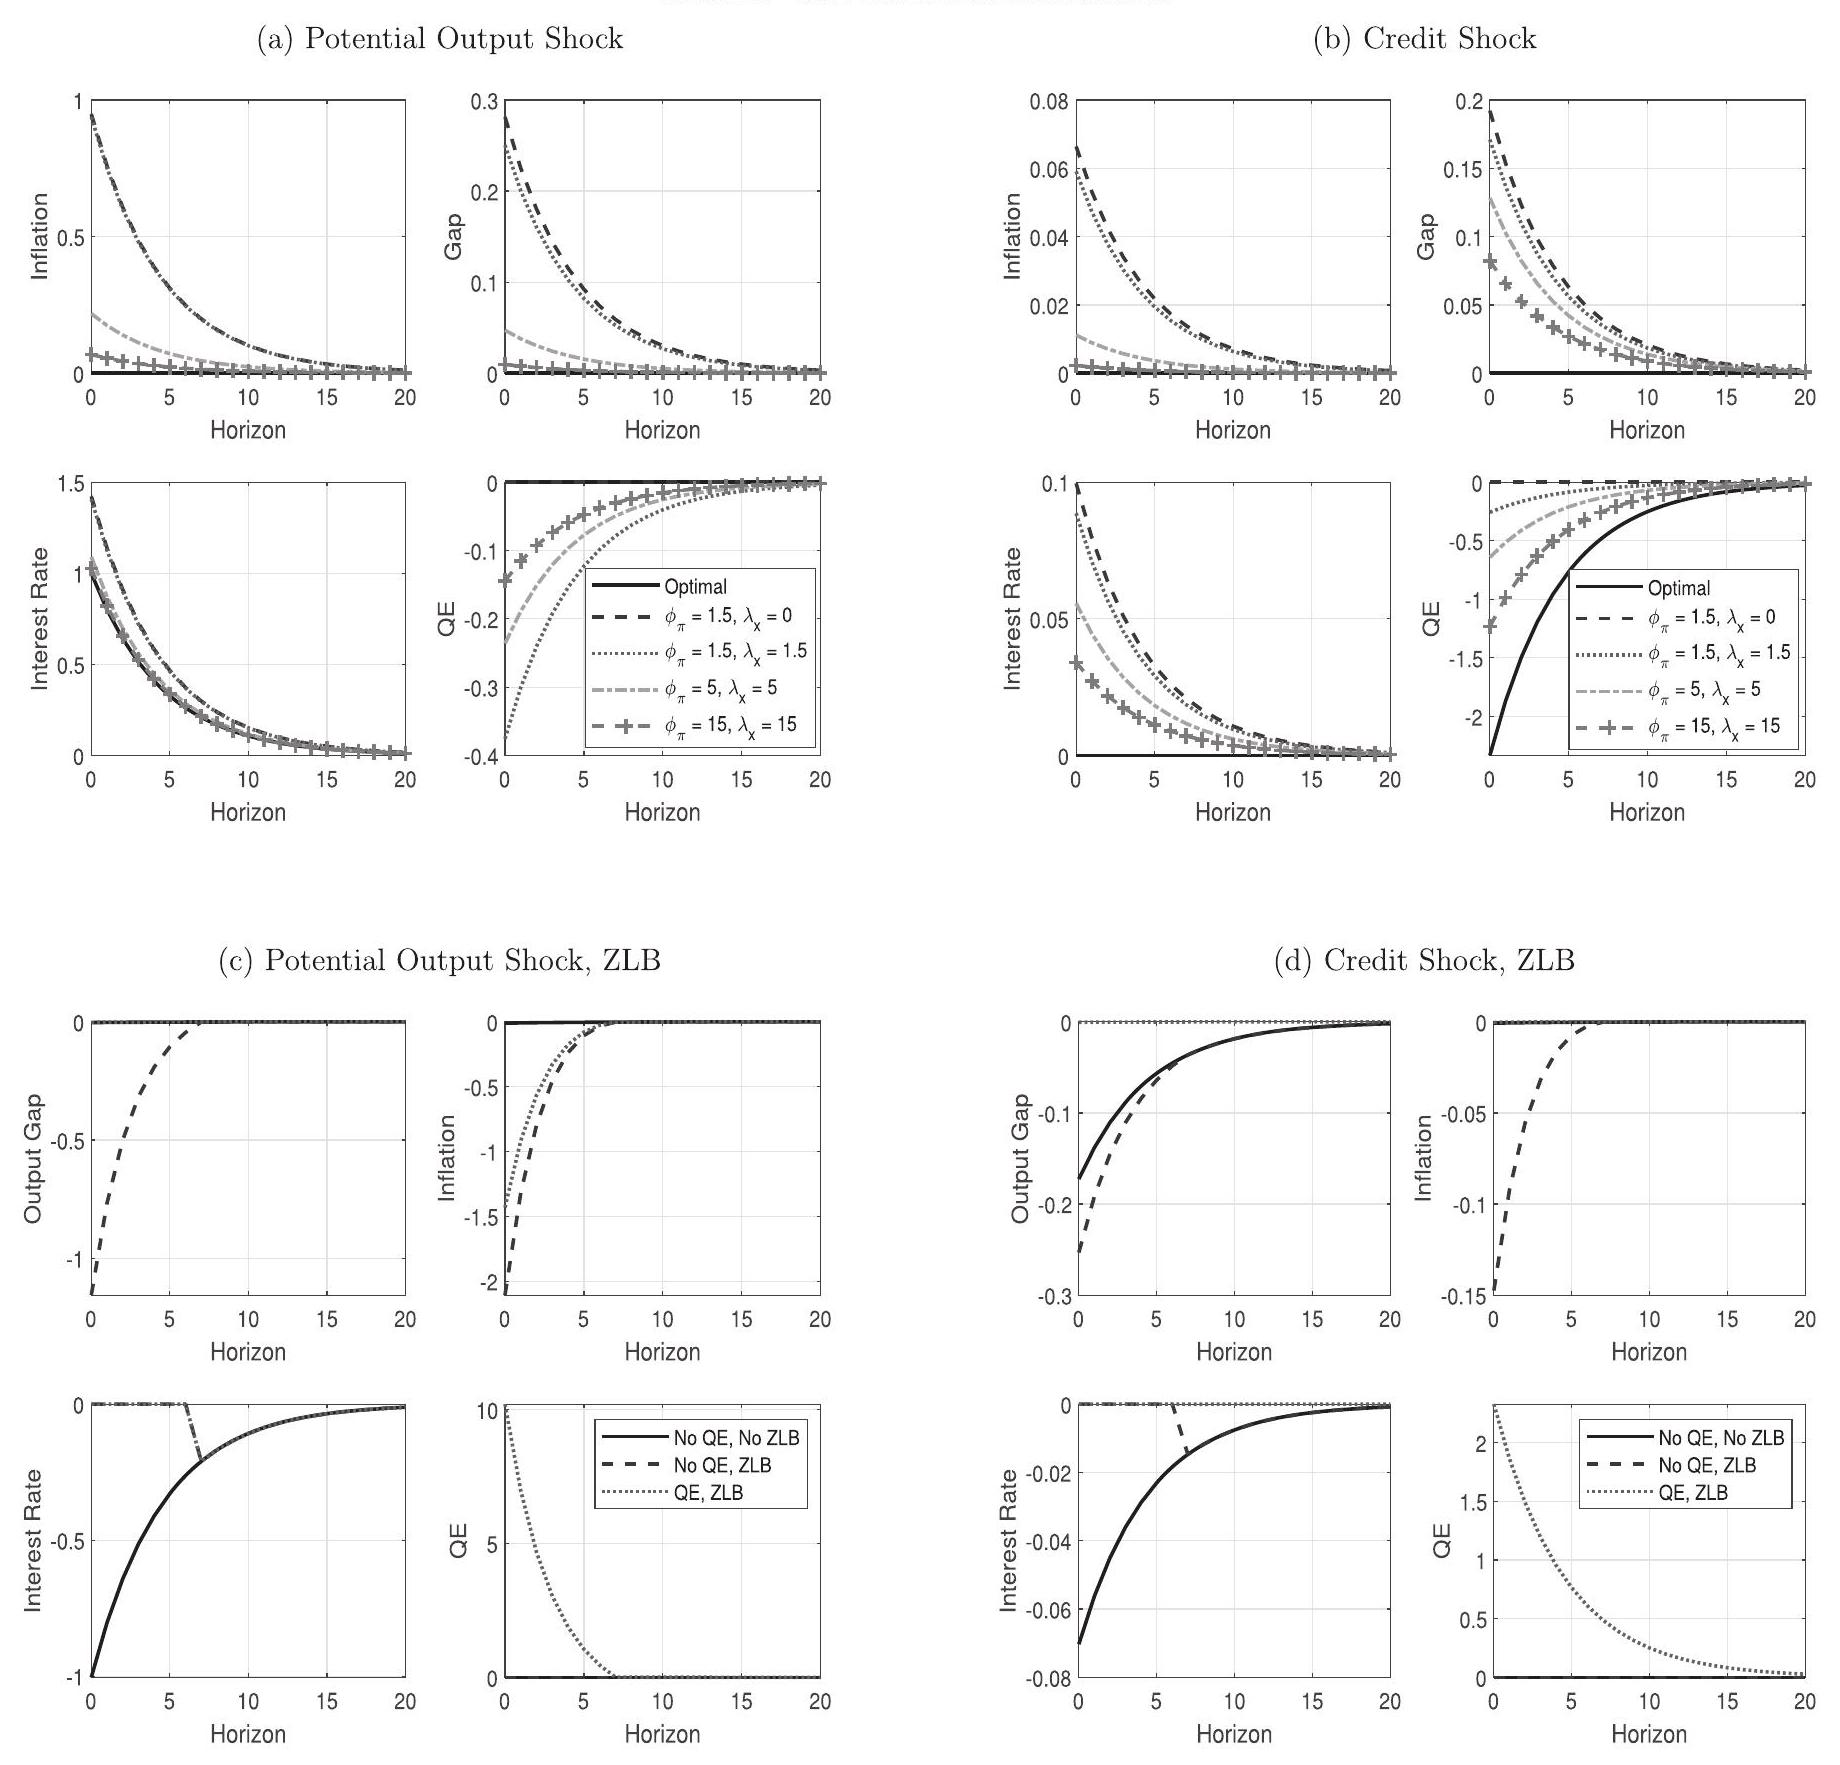
\includegraphics[max width=\textwidth, center]{2024_12_20_098a9c078f922ab7e4b1g-16}

Panels a and b plot impulse responses to a potential output and credit shock, respectively, with different configurations of the rule for the short-term interest rate and QE portfolio, respectively. Panels c and do so when the ZLB on the policy rate is binding. For panels c and d, solid lines show responses when the policy rate obeys a Taylor rule with $\phi_{\pi} \rightarrow \infty$ and $\rho_{r}=\phi_{x}=0$, while QE is constant. Dashed lines depict responses when the ZLB binds for eight quarters, after which time the policy rate reverts to the simple rule; QE remains constant. Dotted lines depict responses when the ZLB binds for eight quarters, but QE follows a simple implementable rule with $\lambda_{x} \rightarrow \infty, \rho_{q}=0$, and $\lambda_{\pi}=0$.

Panel d is constructed similarly to panel c, but considers a contractionary credit shock. The solid line shows responses with no ZLB where the policy rate reacts very strongly to inflation while the central bank's long bond portfolio is fixed. Inflation is stabilized, but the output gap falls. The dashed lines depict responses where QE is again assumed to be held constant, but the ZLB on the policy rate is in place for eight quarters. This results in inflation falling and the gap declining\\
by more than it would absent the ZLB. The dotted lines depict responses when the ZLB on the policy rate binds for eight quarters, but QE follows a rule in which it reacts strongly to the output gap. This necessitates an increase in the central bank's long bond portfolio to offset the credit shock, as shown in the lower-right portion of the figure, but results in both inflation and the gap being completely stabilized. Similar to our result from section III, the ZLB on the policy rate poses\\
no issues for the central bank with regard to credit shocks if QE is optimally implemented.

Our analysis in this section using implementable instrument rules reinforces our results from section III. In particular, QE can be used as an effective albeit imperfect substitute for the short-term policy rate conditional on natural rate shocks. Regardless of the relative weight the central bank attaches on the gap versus inflation, an instrument rule for QE that aggressively targets the output gap results in welfare improvements. Furthermore, a binding ZLB on the policy rate need not pose a problem for the central bank conditional on a credit shock; the same aggressive QE rule can completely stabilize both output and inflation.

\section*{V. Conclusion}
In this paper, we developed a four-equation New Keynesian model with credit shocks, financial intermediation, short- and long-term debt, and a channel for central bank long bond holdings to be economically relevant. The model inherits the tractability and elegance of the benchmark threeequation New Keynesian model. It mainly differs in that credit shocks appear as wedges in both the IS and Phillips curves. In addition to a rule for the short-term policy rate, the fourth equation in the model is a rule for QE .

The model allows us to address the consequences of credit market disturbances as well as the effects of large-scale asset purchases. We produce several analytical results concerning monetary policy design. The presence of credit market frictions breaks the divine coincidence, meaning it is not possible to completely stabilize inflation and the output gap with just one policy instrument. Optimal monetary policy entails adjusting the short-term interest rate to match fluctuations in the natural rate of interest, but manipulating the central bank's long bond portfolio so as to neutralize credit shocks. When it is not possible to adjust the short-term interest (e.g., because of a binding ZLB), credit market shocks need not result in amplified fluctuations if the central bank adjusts its long bond portfolio as it would in normal times. In response to natural rate shocks, adjustment of the central bank's long bond portfolio can serve as a highly effective, albeit imperfect, substitute for conventional policy.

\section*{REFERENCES}
Bauer, Michael D., and Glenn D. Rudebusch, "The Signaling Channel for Federal Reserve Bond Purchases," International Journal of Central Banking 10:3 (2014), s114-s133.\\
Bhattarai, Saroj, Gauti Eggertsson, and Bulat Gafarov, "Time Consistency and Duration of Government Debt: A Model of Quantitative Easing," University of Texas at Austin working paper (2019).\\
Bhattarai, Saroj, and Christopher J. Neely, "An Analysis of the Literature on International Unconventional Monetary Policy," Journal of Economic Literature 20:2 (2020), 527-597.\\
Blanchard, Olivier, and Jordi Galí, "Real Wage Rigidities and the New Keynesian Model," Journal of Money, Credit and Banking 39 (2007), 35-65. 10.1111/j.1538-4616.2007.00015.x

Calvo, Guillermo A., "Staggered Prices in a Utility-Maximizing Framework," Journal of Monetary Economics 12:3 (1983), 383-398. 10.1016/0304-3932(83)90060-0

Carlstrom, Charles, and Timothy Fuerst, "Agency Costs, Net Worth, and Business Fluctuations: A Computable General Equilibrium Analysis," American Economic Review 87:5 (1997), 893-910.\\
Carlstrom, Charles T., Timothy S. Fuerst, and Matthias Paustian, "Fiscal Multipliers under an Interest Rate Peg of Deterministic versus Stochastic Duration," Journal of Money, Credit and Banking 46:6 (2014), 1293-1312. 10.1111/jmcb. 12141

\begin{itemize}
  \item "Targeting Long Rates in a Model with Segmented Markets," American Economic Journal: Macroeconomics 9:1 (2017), 205-242.\\
Chen, Han, Vasco Cúrdia, and Andrea Ferrero, "The Macroeconomic Effects of Large-Scale Asset Purchase Programmes," Economic Journal 122 (2012), F289-F315. 10.1111/j.1468-0297.2012.02549.x\\
Christiano, Lawrence, Martin Eichenbaum, and Sergio Rebelo, "When Is the Government Spending Multiplier Large?," Journal of Political Economy 119:1 (2011), 78-121. 10.1086/659312\\
Clarida, Richard, Jordi Galí, and Mark Gertler, "The Science of Monetary Policy: A New Keynesian Perspective," Journal of Economic Literature 37:4 (1999), 1661-1707. 10.1257/jel.37.4.1661\\
Eggertsson, Gauti B., and Michael Woodford, "The Zero Bound on Interest Rates and Optimal Monetary Policy," Brookings Papers on Economic Activity 34:1 (2003), 139-235. 10.1353/eca.2003.0010\\
Galí, Jordi, Monetary Policy, Inflation, and the Business Cycle: An Introduction to the New Keynesian Framework (Princeton, NJ: Princeton University Press, 2008).\\
Gertler, Mark, and Peter Karadi, "A Model of Unconventional Monetary Policy," Journal of Monetary Economics 58:1 (2011), 17-34. 10.1016/j.jmoneco.2010.10.004\\
— "QE 1 vs. 2 vs. 3 . . : A Framework for Analyzing Large-Scale Asset Purchases as a Monetary Policy Tool," International Journal of Central Banking 9:S1 (2013), 5-53.\\
Guerrieri, Luca, and Matteo Iacoviello, "OccBin: A Toolkit for Solving Dynamic Models with Occasionally Binding Constraints Easily," Journal of Monetary Economics 70 (2015), 22-38. 10.1016/ j.jmoneco.2014.08.005
\end{itemize}

Hamilton, James D., and Jing Cynthia Wu, "The Effectiveness of Alternative Monetary Policy Tools in a Zero Lower Bound Environment," Journal of Money, Credit, and Banking 44:s1 (2012), 3-46. 10.1111/j.1538-4616.2011.00477.x

Mau, Ronald, "Purchases and Sales of Long Bonds as a Monetary Policy Instrument," University of Mississippi working paper (2019).\\
Schmitt-Grohe, Stephanie, and Martin Uribe, "Optimal Simple and Implementable Monetary and Fiscal Rules," Journal of Monetary Economics 554:5 (2007), 1702-1725. 10.1016/j.jmoneco.2006.07.002\\
Sims, Eric, and Jing Cynthia Wu, "Are QE and Conventional Monetary Policy Substitutable?," International Journal of Central Banking 16:1 (2020a), 195-230.\\
\_ \_Wall Street vs. Main Street QE," NBER working paper 27295 (2020b).

\begin{itemize}
  \item "Evaluating Central Banks' Tool Kit: Past, Present, and Future," Journal of Monetary Economics 185 (2021), 135-160. 10.1016/ j.jmoneco.2020.03.018
\end{itemize}

Smets, Frank, and Rafael Wouters, "Shocks and Frictions in US Business Cycles: A Bayesian DSGE Approach," American Economic Review 97:3 (2007), 586-606. 10.1257/aer.97.3.586\\
Tinbergen, Jan, On the Theory of Economic Policy (Amsterdam: NorthHolland, 1952).\\
Vayanos, Dimitri, and Jean-Luc Vila, "A Preferred-Habitat Model of the Term Structure of Interest Rates," London School of Economics working paper (2009).\\
Wallace, Neil, "A Modigliani-Miller Theorem for Open-Market Operations," American Economic Review 71:3 (1981), 267-274.\\
Woodford, Michael, Interest and Prices: Foundations of a Theory of Monetary Policy (Princeton, NJ: Princeton University Press, 2003).\\
Wu, Jing Cynthia, and Fan Dora Xia, "Measuring the Macroeconomic Impact of Monetary Policy at the Zero Lower Bound," Journal of Money, Credit, and Banking 48:2-3 (2016), 253-291. 10.1111/ jmcb. 12300


\end{document}